\PassOptionsToPackage{table,dvipsnames}{xcolor}   % must come before the class
\documentclass[sigconf,nonacm]{acmart}
% ================= PREAMBLE =================
\sloppy

% Math, symbols
% \usepackage{amssymb}
\usepackage{pifont}
\usepackage[mathcal]{euscript}
\newcommand{\cmark}{\ding{51}}
\newcommand{\xmark}{\ding{55}}
\usepackage{placeins}

% Tables, colors
\usepackage{float}
\usepackage{hhline}
\usepackage{makecell}
\usepackage[most]{tcolorbox}
\usepackage{threeparttable}

% Figures
\usepackage{subcaption}
\usepackage{tikz}
\usepackage{standalone}
\usetikzlibrary{arrows.meta,shapes.geometric}

% Algorithms
\usepackage[ruled,vlined]{algorithm2e}
\usepackage{algpseudocode}

% Floats and page layout
\usepackage{xurl}

% Text and lists
\usepackage{enumitem}

% Numbers and units
\usepackage[
  separate-uncertainty = true,
  multi-part-units = repeat
]{siunitx}

% Tables: flexible and dashed-line support
\usepackage{adjustbox}
\usepackage{array}
\usepackage{longtable}
\usepackage{tabularx}
\usepackage{ragged2e}
\newcolumntype{Y}{>{\raggedright\arraybackslash}X}
\usepackage{arydshln}
\usepackage{multirow}

% ================= CUSTOM FORMATTING =================
\newtcolorbox{GrayBox}[2][]{%
  enhanced,
  float=htbp,
  width=\columnwidth,
  colback=gray!10,
  colframe=black!70,
  arc=1mm,
  boxrule=0.5pt,
  left=1ex,
  right=1ex,
  top=0.5ex,
  bottom=0.5ex,
  before skip=4pt,
  after skip=4pt,
  title=#2,
  #1
}

\newcommand{\dsc}[1]{%
  \par\medskip
  \noindent\textbf{#1}\par\vspace{0.5em}
}

\newcommand{\parg}[1]{%
  \par\medskip \noindent\textbf{\textit{#1}}\quad%
}

\newcommand{\best}[1]{\cellcolor{gray!25}{#1}}
\newcommand{\nb}[1]{\cellcolor{pink!30}{#1}}
\definecolor{gainbase}{HTML}{A6CEE3}
\definecolor{lossbase}{HTML}{CAB2D6}
\newcommand{\gc}[1]{\cellcolor{gainbase!#1!white}}
\newcommand{\rc}[1]{\cellcolor{lossbase!#1!white}}

% ================= MODEL SHORTHANDS =================
\newcommand{\zs}{UXC\textsubscript{ZS}}
\newcommand{\ft}{UXC\textsubscript{FT}}
\newcommand{\mlp}{$\mathcal{N}$\textsubscript{MLP}}
\newcommand{\f}[1]{#1$_{\text{F}}$}
\newcommand{\ff}[1]{#1$_{\text{FF}}$}
\newcommand{\fm}[1]{#1$_{\text{FM}}$}
\newcommand{\ffm}[1]{#1$_{\text{FFM}}$}
\newcommand{\uhgt}{HGT{-U}}

% ================= PAPER METADATA =================
\newcommand{\paperabstract}{%
Code-to-architecture mapping assigns source files to modules of a reference architecture. Representations of implementation artifacts can capture code text, dependencies, and directory organization, but predictive gains alone do not establish the contribution of additional graph processing. Dependencies may already be encoded in these representations, while directories may closely match the reference decomposition. We investigate how artifact representations and graph context affect mapping on ten Java, C, and C++ systems with a limited labeling budget. We compare lexical, structural, and contextual file representations and assess each predictor with and without dependency neighbors. Using a Heterogeneous Graph Transformer (HGT), we compare file-level graphs extended with member nodes summarizing each file’s program elements, folder nodes, or both, alongside a variant encoding folder paths directly in file representations. We compare folder-aware predictions with a directory rule using the same labeled files.

Representations encoding dependency information outperform lexical representations on most systems. Additional neighbor aggregation can improve mapping, depending on the predictor and aggregation direction. Folder-aware variants yield the largest and most consistent gains across the evaluated HGT configurations. However, the directory rule achieves per-system median accuracy of 89–100\%, and adding folder information does not consistently improve predictions for files the rule misclassifies. Member nodes provide no consistent improvement over file-level graphs. These findings support assessing what file representations and directory organization already provide before attributing improvements to graph neural networks.
}

% ================= TITLE, AUTHORS, ABSTRACT =================
\title{What Carries Architectural Signal? A Code-to-Architecture Mapping Study}

\author{Rakhshanda Jabeen}
\affiliation{\institution{Electrolux Professional AB}\city{Ljungby}\country{Sweden}}
\affiliation{\institution{Linnaeus University}\city{V\"axj\"o}\country{Sweden}}
\email{rakhshanda.jabeen@electroluxprofessional.com}

\author{Morgan Ericsson}
\affiliation{\institution{Linnaeus University}\city{V\"axj\"o}\country{Sweden}}
\email{morgan.ericsson@lnu.se}

\author{Yuyao Duan}
\affiliation{\institution{Linnaeus University}\city{V\"axj\"o}\country{Sweden}}
\email{yuyaoduan4@gmail.com}

\author{Anna Wingkvist}
\affiliation{\institution{Linnaeus University}\city{V\"axj\"o}\country{Sweden}}
\email{anna.wingkvist@lnu.se}

\begin{abstract}
\paperabstract
\end{abstract}

\keywords{Code-to-Architecture Mapping, Software Architecture, Graph Neural Networks, Heterogeneous Graphs, Representation Learning}

% ================= DOCUMENT =================
% ================= DOCUMENT =================
\begin{document}
\makeatletter
\renewcommand\subsubsection{%
  \@startsection{subsubsection}{3}{\z@}%
    {-1.5ex plus -0.5ex minus -0.2ex}%
    {0.5ex plus 0.2ex}%
    {\normalfont\normalsize\itshape}%
}
\let\ACM@origsubsubsection\subsubsection
\makeatother

\raggedbottom
\maketitle

\section{Introduction\label{sec:intro}}

Maintaining a software architecture requires knowing which implementation elements belong to its modules. That correspondence can become difficult to maintain as a system grows: new files introduce responsibilities and dependencies, while architectural documentation may lag behind the implementation. Code-to-architecture (C2A) mapping addresses this problem by assigning source files to the modules of a reference architecture. The resulting mapping supports reflexion modeling, which compares implementation dependencies with architectural relations to identify divergence~\cite{reflexion1}. It therefore connects the modular decomposition used to reason about a system~\cite{parnas1972,clements2003} to the code in which that decomposition is realized.
 
Several sources of evidence can support a mapping. Identifiers express domain concepts and implementation roles. Contextual code representations capture information from declarations and operations. Static dependencies locate a file among other files with which it interacts, while directories record how developers organize the project~\cite{sarif,negar,garcia2013}. These sources need not agree: a utility may depend on several modules, terminology may be shared across responsibilities, and a directory may contain files assigned to different architectural modules.
 
The usefulness of an information source also depends on how it enters a predictor. A dependency embedding can encode graph structure before a classifier sees a file. Propagating over dependencies then supplies a second form of access to related files, with its own assumptions about direction, relation types, and aggregation. A gain from the embedding does not establish that this additional propagation will help. Similarly, a folder-aware model can improve overall agreement with a reference architecture while losing correct predictions for files that depart from a directory-based assignment. These distinctions motivate studying both the information supplied to a model and the changes caused by the way it processes that information.

Prior architecture recovery and mapping work provides several ways to represent these sources. NEGAR learns structural representations using Node2Vec random walks on the dependency graph~\cite{negar}; GAER used a graph autoencoder with Word2Vec identifier embeddings for recovery~\cite{gaer}; prior mapping work uses lexical and organizational features with graph convolutional networks~\cite{jabeen2025graph}. Later work compares random walk-based methods with graph attention and diffusion-based rewiring and examines alternative uses of dependencies and folders~\cite{structsar}. These studies generally fix the representation chosen for each source, so it remains unclear which signal provides the strongest architectural evidence and how it should be represented.

We study this question through C2A mapping, a prerequisite for reflexion modeling~\cite{reflexion1}. We formulate C2A mapping as a classification problem in which each file is assigned to one module of the reference architecture. We work in a low-label setting, where about 5\% of the files are already mapped, and the model infers the remaining assignments. The model is trained either on the labeled files alone or with self-training using its own confident predictions. This setting allows us to examine how file representations and graph relations contribute under limited supervision.

Our evaluation uses ten Java, C, and C++ systems and covers lexical Word2Vec, structural Node2Vec, and contextual UniXcoder representations. These serve as inputs to a graph-free neural baseline and to two graph neural networks (GNNs), a Heterogeneous Graph Transformer (HGT)~\cite{hgt} and, in the controlled comparisons, a Graph Attention Network (GAT)~\cite{gat}. The heterogeneous configurations contain file nodes and, where applicable, folder nodes and one aggregate member node per file. They vary both the context available to a file and where feature content is stored. We compare these file representations and complement the configuration comparisons with controlled comparisons that change one design choice while holding the features, labeled splits, initialization, and training budgets fixed within each comparison.
 
The configuration results motivate two complementary analyses. A directory analysis distinguishes errors corrected by a model from previously correct predictions that it makes incorrect. A dependency analysis first tests whether embeddings retain useful information beyond a degree-preserving rewiring control on three systems, then compares ways of using dependency neighbors on all nine systems. Both stages of the dependency analysis use supervised-only and self-training schedules of equal duration.

We address three research questions:
\begin{itemize}
    \item \textbf{RQ1.} How does mapping performance vary across lexical, structural and contextual file representations?
    \item \textbf{RQ2.} How does mapping performance change when those representations are used in file, member, and folder graph configurations?
    \item \textbf{RQ3.} How do graph representation, training schedule, and neighbor processing affect the contribution of structural context?
\end{itemize}

The results show that dependency information supports C2A mapping through both file representations and neighbor context, but the benefit of neighbor context depends on how it is processed. Folder organization yields the largest gains, largely reflecting information already available through a directory rule. Aggregate improvements can conceal regressions on individual files. These findings clarify how input signals and their use by a predictor affect C2A mapping across the nine systems studied\footnote{\label{fn:code}Code and data are available at \url{https://github.com/sse-lnu/hetmap}.}.
%\section{Background \label{sec:background}}

Software artifacts are naturally relational and multi-typed. A system contains folders, source files or classes, and finer-grained program elements such as methods and fields, connected through relations that include folder containment, file-to-member composition, and static code-level dependencies.

To preserve these distinctions, we represent each software system as a typed graph:
$$G=(V, E,\mathcal{A},\mathcal{R}),$$
where $V$ and $E$ are the sets of artifact nodes and relations between them, respectively. The mappings $\tau: V \rightarrow \mathcal{A}$ and $\phi: E \rightarrow \mathcal{R}$ assign node and relation types. In our most detailed configuration, $\mathcal{A}$ contains folder, file, and aggregate member types, while $\mathcal{R}$ distinguishes folder containment, file-to-member composition, and a single dependency relation that merges all file-level static dependencies. The file-level graph is homogeneous, and adding folder or member nodes makes it heterogeneous.

A relation's meaning depends on its type and the types of its source and target nodes in $G$. We describe an edge $e_{s,t}$ from node $s$ to node $t$ by the meta-relation $\langle \tau(s), \phi(e_{s,t}), \tau(t) \rangle$. For example, $\langle \text{folder}, \text{contains}, \text{file} \rangle$ captures project organization, whereas $\langle \text{file}, \text{depends on}, \text{file} \rangle$ captures code-level coupling. These meta-relations preserve the distinction between structural organization and implementation dependencies, which a homogeneous graph with one node type and one relation type does not explicitly represent.

HGT~\cite{hgt} exploits such meta-relations during message passing by conditioning attention and message transformation on the source node type, edge type, and target node type. GAT~\cite{gat} also uses attention-based message passing, but its standard formulation does not explicitly distinguish node or relation types. HGT can also operate on a graph with a single node type and a single relation type, although this does not make its attention mechanism equivalent to that of GAT.

The initial node features determine what information is available before message passing, while graph structure determines which nodes exchange information. Depending on how they are encoded, a file's features can capture lexical evidence from its identifiers, structural evidence from its position in the dependency graph, or contextual evidence from its code.

A lexical embedding trained on identifier tokens captures naming patterns but does not explicitly encode dependency structure or implementation syntax and behavior. A graph embedding such as Node2Vec~\cite{node2vec} instead encodes structural neighborhoods without using code content. Such embeddings have been used to capture dependency-based cohesion in architecture recovery~\cite{negar,structsar}.

Contextual representations from pretrained code encoders such as UniXcoder~\cite{unixcoder} capture the syntactic and behavioral content of an implementation that lexical features miss, but their pretraining objectives do not target architectural grouping: files with similar code can belong to different modules. Contrastive learning adapts an encoder to a chosen notion of similarity by bringing designated positive pairs closer than other in-batch examples treated as negatives, using an InfoNCE objective~\cite{infonce}. Dependency-derived positive pairs encourage embeddings to reflect dependency proximity, which need not align with reference-module membership.
\section{Methodology\label{sec:method}}

This section presents the methodology for studying how architectural signals and graph design choices affect code-to-architecture mapping. We formulate the mapping task as node classification over a software graph $G=(V, E,\mathcal{A},\mathcal{R})$, where $\mathcal{A}$ and $\mathcal{R}$ denote the sets of node and relation types. Let $V_f \subseteq V$ be the set of file nodes, which are the targets of the mapping task. A small subset $L \subset V_f$ is initially labeled with known architectural module assignments, and the remaining file nodes $U = V_f \setminus L$ are unlabeled. The objective is to learn an encoder:
\begin{equation}
Z = f_{\theta}(G), \qquad Z \in \mathbb{R}^{|V_f| \times d},
\end{equation}
that maps each source file $i\in V_f$ to a $d$-dimensional embedding $z_i$, where $\theta$ denotes the learnable parameters of the representation-learning method. These file embeddings are used to predict architectural modules and to infer the labels of the nodes in $U$.
 
We first describe the graphs and the structural, lexical, and contextual features used to initialize their nodes. We then present the graph-free MLP, the HGT encoder, and their iterative training procedure. RQ1 varies the file representation, using the graph-free MLP. RQ2 varies the graph configuration for each representation and compares the results with a directory baseline described in Section~\ref{sec:dir_predictor}. RQ3 fixes the representations and varies neighbor information, predictor, and training schedule, as described in Section~\ref{sec:controlled_setup}.

 % _______ Graph Construction ___________
\subsection{Heterogeneous Graph Construction\label{sec:het_graph}}
We model the software system as a heterogeneous graph whose nodes represent software artifacts and edges represent organizational, containment, and dependency relations. The graph is built from three sources of information: the folder structure of the project, the containment of program elements within a file, and static dependencies extracted from source code. Folder structure provides organizational context, containment connects folders to the files they contain and members to the files they belong to, and static dependencies describe interactions between software entities. We preserve these sources as distinct node and relation types rather than collapsing them into a single homogeneous graph. Figure~\ref{fig:schema} illustrates the general schema of the heterogeneous software graph and the meta-relations used in our model.
 
\begin{figure}[!h]
\centering
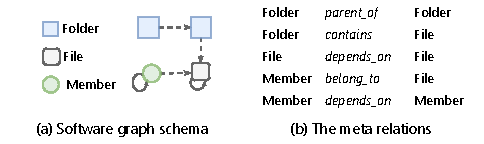
\includegraphics[width=1\linewidth]{Images/hetmap_schema.pdf}
\caption{Schema and meta-relations of the heterogeneous software graph. The figure shows the most expressive representation, with folder, file, and member nodes. Simpler variants remove selected node types or aggregate member-level dependencies at the file level.\label{fig:schema}}
\end{figure}
 
\subsubsection{Node Types}
We use three node types: folder, file, and member. Folder nodes represent directory levels in the project structure. File nodes represent source files and are the target nodes for code-to-architecture mapping. Member nodes represent member-level program information associated with a file, including methods, fields, constructors, and variables.
 
We use one summarized \textit{Member} node per file rather than representing each method, field, constructor, or variable as a separate node. The member node aggregates lexical and dependency information from the members of its associated file, retaining member-level information while avoiding the large and sparse graphs produced by fully fine-grained representations.

\subsubsection{Relation Types}
The graph contains structural relations, including organization, containment, and dependency. Logical components are often implemented through namespaces or directory structures that group source code providing a particular functionality, and such structures reflect how developers organize files~\cite{fundamentals_sa, garcia2013}. To preserve this information, each directory level is represented as a separate folder node. Folder nodes are connected through \emph{parent\_of} edges, forming hierarchical chains such as \texttt{app} $\rightarrow$ \texttt{app/ui} $\rightarrow$ \texttt{app/ui/views}. File nodes are linked to their folder through \emph{contains} edges, and each member node is connected to its enclosing file through a \emph{belongs\_to} edge.

Static dependencies provide direct evidence of how entities interact and are a central source of information for architecture mapping and recovery~\cite{negar, deps_impact}. The frozen dependency artifacts were extracted with the Depends tool~\cite{depends}, which analyzes the syntactic structure of the projects studied in this paper and identifies entities together with several categories of static relations. Different dependency types can carry distinct architectural meanings~\cite {edge_weights, sarif}, so we keep them as separate relational edge types rather than merging them into a single dependency relation. Table~\ref{tab:relation_types} lists the structural relations introduced during graph construction and the static dependency types observed in the analyzed Java and C/C++ systems.

\begin{table}[htb]
\centering
\caption{Structural and static dependency relation types used in the software graph.}
\label{tab:relation_types}

\renewcommand{\arraystretch}{1}
\begin{adjustbox}{max width=\columnwidth}
\begin{threeparttable}
\begin{adjustbox}{max width=\columnwidth}
\begin{tabular}{ll}
\toprule
\textbf{Relation type} & \textbf{Description} \\
\midrule
\emph{parent\_of} & Folder contains a subfolder in the directory. \\
\emph{contains} & Folder contains a source file. \\
\emph{belongs\_to} & Member-level program element belongs to a file. \\
\midrule
\texttt{Call} & Function or method invocation. \\
\texttt{Cast} & Conversion of an entity to another type. \\
\texttt{Contain} & Definition or containment of variables/fields. \\
\texttt{Create} & Creation of an instance or program entity. \\
\texttt{Extend} & Inheritance or parent-child type relation. \\
\texttt{Implement} & A class implements an interface or abstraction. \\
\texttt{Import} & A file imports other classes, methods, or variables. \\
\texttt{Parameter} & Use of a type as a method or function parameter. \\
\texttt{Return} & Use of a type as a return type. \\
\texttt{Use} & Use or assignment of variables. \\
\bottomrule
\end{tabular}
\end{adjustbox}
\begin{tablenotes}[flushleft]
\item \texttt{Annotation} and \texttt{Throw} are not observed in the C/C++ systems.
\end{tablenotes}
\end{threeparttable}
\end{adjustbox}
\end{table}

\subsubsection{Graph Variants\label{sec:graph_variants}}
Folder organization, member-level information, and static dependencies are available simultaneously in the complete graph, so their contributions cannot be determined from the full configuration alone. We therefore construct four graph variants that vary the presence of folder and member nodes while retaining dependency information at the available granularity. Figure~\ref{fig:graph_variants_overview} provides a visual overview; Table~\ref{tab:graph_variants} summarizes their roles. Files are always the prediction targets. A member node summarizes a file's program members, while folder nodes supply directory context.

\begin{figure}[tb]
\centering
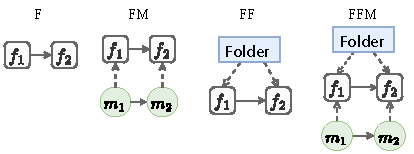
\includegraphics[width=1\linewidth]{Images/graph_variants.pdf}
\caption{Graph configurations: files $f_i$ are the prediction targets; each $m_i$ aggregates the members of file $f_i$. Solid arrows show dependencies and dashed arrows show meta-relations. The panels omit relation types, additional dependency edges, and folder ancestry; Figure~\ref{fig:schema} gives the typed schema. Feature construction also depends on the configuration, as described in Section~\ref{sec:node_features}.\label{fig:graph_variants_overview}}
\end{figure}

We classify dependencies according to their resolved endpoints. A dependency is file-level if at least one endpoint is a file; this includes file--file, file--member and member--file interactions. It is member-level if both endpoints are members. FFM keeps these dependency edges separate from containment relations and preserves their endpoint types. FM removes folder nodes and relations while retaining files and members. FF and F also remove member nodes. In these variants, each member endpoint is replaced by its enclosing file, so all remaining dependencies connect file nodes.

\begin{table}[!ht]
\centering
\caption{Graph variants used to study the effect of graph granularity and information sources.}
\label{tab:graph_variants}
\begin{adjustbox}{max width=\columnwidth}
\Large
\begin{tabular}{l l l}
\toprule
\textbf{Variant} & \textbf{Node types} & \textbf{Purpose} \\
\midrule
FFM & Folder, File, Member & Complete heterogeneous structure \\
FF & Folder, File & Folder and file-level structure \\
FM & File, Member & Member-level structure without folders \\
F & File & File-level dependency baseline \\
\bottomrule
\end{tabular}
\end{adjustbox}
\end{table}
% _________ Node Feature Initialization ______________

\subsubsection{Relation Types}
The graph contains structural relations, including organization, containment, and dependency. Logical components are often implemented through namespaces or directory structures that group source code providing a particular functionality, and such structures reflect how developers organize files~\cite{fundamentals_sa, garcia2013}. To preserve this information, each directory level is represented as a separate folder node. Folder nodes are connected through \emph{parent\_of} edges, forming hierarchical chains such as \texttt{app} $\rightarrow$ \texttt{app/ui} $\rightarrow$ \texttt{app/ui/views}. File nodes are linked to their folder through \emph{contains} edges, and each member node is connected to its enclosing file through a \emph{belongs\_to} edge.
 
Static dependencies provide direct evidence of how entities interact and are a central source of information for architecture mapping and recovery~\cite{negar, deps_impact}. Dependencies were extracted with the Depends tool~\cite{depends}, which analyzes the syntactic structure of the projects studied in this paper and identifies entities together with several categories of static relations. Different dependency types can carry distinct architectural meanings~\cite{edge_weights, sarif}, so we keep them as separate relational edge types rather than merging them into a single dependency relation. Table~\ref{tab:relation_types} lists the structural relations introduced during graph construction and the static dependency types observed in the analyzed Java and C/C++ systems.
 
\begin{table}[htb]
\centering
\caption{Structural and static dependency relation types used in the software graph.}
\label{tab:relation_types}
 
\renewcommand{\arraystretch}{1}
\begin{adjustbox}{max width=\columnwidth}
\begin{threeparttable}
\begin{adjustbox}{max width=\columnwidth}
\begin{tabular}{ll}
\toprule
\textbf{Relation type} & \textbf{Description} \\
\midrule
\emph{parent\_of} & Folder contains a subfolder in the directory. \\
\emph{contains} & Folder contains a source file. \\
\emph{belongs\_to} & Member-level program element belongs to a file. \\
\midrule
\texttt{Call} & Function or method invocation. \\
\texttt{Cast} & Conversion of an entity to another type. \\
\texttt{Contain} & Definition or containment of variables/fields. \\
\texttt{Create} & Creation of an instance or program entity. \\
\texttt{Extend} & Inheritance or parent-child type relation. \\
\texttt{Implement} & A class implements an interface or abstraction. \\
\texttt{Import} & A file imports other classes, methods, or variables. \\
\texttt{Parameter} & Use of a type as a method or function parameter. \\
\texttt{Return} & Use of a type as a return type. \\
\texttt{Use} & Use or assignment of variables. \\
\bottomrule
\end{tabular}
\end{adjustbox}
\begin{tablenotes}[flushleft]
\item \texttt{Annotation} and \texttt{Throw} are not observed in the C/C++ systems.
\end{tablenotes}
\end{threeparttable}
\end{adjustbox}
\end{table}
 
\subsubsection{Graph Variants\label{sec:graph_variants}}
Folder organization, member-level information, and static dependencies are available simultaneously in the complete graph, so their contributions cannot be determined from the full configuration alone. We therefore construct four graph variants that vary the presence of folder and member nodes while retaining dependency information at the available granularity. Figure~\ref{fig:graph_variants_overview} provides a visual overview. Files are always the prediction targets, a member node summarizes a file's program members, and folder nodes supply directory context.
 
\begin{figure}[tb]
\centering
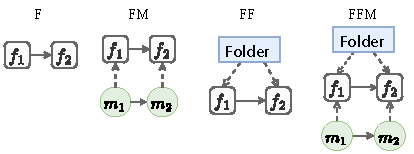
\includegraphics[width=1\linewidth]{Images/graph_variants.pdf}
\caption{\small Graph configurations: files $f_i$ are the prediction targets; each $m_i$ aggregates the members of file $f_i$. Solid arrows show dependencies and dashed arrows show meta-relations. The panels omit relation types, additional dependency edges, and folder ancestry; Figure~\ref{fig:schema} gives the typed schema. Feature construction also depends on the configuration, as described in Section~\ref{sec:node_features}.\label{fig:graph_variants_overview}}
\end{figure}
 
We classify dependencies according to their resolved endpoints. A dependency is file-level if at least one endpoint is a file; this includes file--file, file--member, and member--file interactions. It is member-level if both endpoints are members. FFM is the complete graph and keeps these dependency edges separate from containment relations, preserving their endpoint types. FM removes folder nodes and relations while retaining files and members. FF removes member nodes instead, and F removes both folder and member nodes and serves as the file-level dependency baseline. In FF and F, each member endpoint is replaced by its enclosing file, so all remaining dependencies connect file nodes. The controlled experiments also use a homogeneous version of F, in which dependency direction and edge types are removed.
 
% _________ Node Feature Initialization ______________
\subsection{Node Feature Initialization \label{sec:node_features}}
We initialize node features based on the information source used in each experimental setting. Folder nodes are always initialized from binary folder-path tokens, regardless of which strategy is used elsewhere in the graph. File and member nodes are initialized using one of three strategies: lexical embeddings from Word2Vec, structural embeddings from Node2Vec, or contextual embeddings from UniXcoder, used zero-shot or fine-tuned with dependencies as described below.
 
\subsubsection{Folder Node Features}
 
Folder nodes are encoded using a binary bag-of-words representation over folder tokens. The folder tokens are derived from directory segments after removing common project-root tokens. Each folder node is represented by the tokens along its path in the directory hierarchy. For example, a folder corresponding to \texttt{app/ui/views} carries the tokens \texttt{app}, \texttt{ui}, and \texttt{views}. This allows deeper folder nodes to retain information about their hierarchical context.
 
\subsubsection{Word2Vec: Lexical Features \label{sec:node_w2v}}
Source code identifiers often encode domain concepts and implementation roles, making them useful cues for mapping entities to architectural modules~\cite{sarif}. We use Word2Vec embeddings following the approach of Jabeen et al.~\citep{gaer} for lexical input. Tokens are extracted from file names and member-level program elements, including methods, fields, constructors, and variables. We normalize identifiers by splitting camelCase, PascalCase, and snake\_case forms, converting tokens to lowercase, and removing stopwords and non-alphabetic tokens. The remaining tokens are represented using 128-dimensional skip-gram Word2Vec embeddings~\cite{word2vec}, trained for 20 epochs with a context window of five. Each node representation is computed by averaging the embeddings of its associated tokens.
 
The graph variant determines where these features are stored. In FFM and FM, the file node contains file-name tokens and the member node contains identifiers from the file's program elements. FF and F have no member nodes, so member identifiers are included in the file representation instead, and the graph-free MLP uses the same file vector as F and FF. Member identifiers therefore remain available in every variant, but moving to FM or FFM changes where the information enters the model as well as changing the graph and its parameters.
 
\subsubsection{Node2Vec: Structural Features \label{sec:node_n2v}}
Chen et al.~\citep{negar} observe that files in the same architectural module can occupy a dense local dependency region without being directly connected. Shallow message passing over raw dependency graphs can therefore provide too limited a context to expose such relationships, whereas random walks can capture longer-range dependency structure~\cite{structsar}. We use Node2Vec's~\cite{node2vec} random-walk embeddings as a structural initialization and merge all static dependency types into a single edge type before generating random walks. Its biased random walks use parameters $p$ and $q$ to balance local and exploratory walks. The resulting embeddings capture structural similarity from dependency position without using identifier text or folder location.
 
In FM and FFM, each aggregate member node receives the Node2Vec embedding of its corresponding file. These configurations therefore change graph processing without introducing a separately learned member-level structural embedding.
 
\subsubsection{UniXcoder: Contextual Features \label{sec:unixcoder}}
For contextual initialization, we use UniXcoder~\cite{unixcoder}, a pretrained code transformer. The zero-shot variant uses its pretrained weights directly. The dependency-guided variant fine-tunes the encoder separately for each system using that system's dependency structure.
 
Source files are parsed with tree-sitter~\cite{tree_sitter} to produce separate file and member views. For Java, the file view contains type headers, field declarations, and constructor signatures with short body excerpts. The member view contains ordinary method declarations and excludes constructors. C/C++ extraction uses the appropriate language grammars to separate type and state declarations, including applicable constructors, from ordinary operations. It preserves physical-file boundaries and does not expand includes or macros. Unlike Word2Vec, UniXcoder does not move the member text into the file view when member nodes are absent.
 
Jabeen et al.~\cite{structsar} show that shallow message passing over the raw dependency graph struggles to expose relationships between files that are connected only through shared neighbors rather than a direct edge. Therefore, positive pairs for contrastive fine-tuning are drawn primarily from the two-hop neighborhood: for each anchor file, two-hop candidates are ranked by the number of distinct one-hop neighbors shared with the anchor, and two pairs per file are sampled from the top eight candidates; files without any two-hop candidates fall back to a direct neighbor. Training uses an InfoNCE~\cite{infonce} objective with in-batch negatives; in-batch items connected by dependencies but not selected as a positive pair are masked so that they act as neither positive nor negative.
 
Only the upper four encoder layers are updated during fine-tuning, while the token embedding layer and the lower eight encoder layers stay frozen, since the number of dependency pairs available in a single system is small relative to the encoder's parameter count. Adaptation is performed independently for each subject system, as dependency structure and naming conventions are project-specific.
 
Member information therefore enters the model differently for each representation. W2V moves member identifiers from the file vector to the member node when member nodes are present, UniXcoder provides member text only through the member node, and N2V gives the member node the file's own vector. Moving from F to FM or FFM thus changes how information enters the model as well as the graph, and the comparisons across graph variants are interpreted for each representation separately.
% __________ Model ________________
\subsection{Mapping Models\label{sec:mapping_models}}
All models map the final file representation to module logits with a linear layer and are trained by minimizing categorical cross-entropy over the labeled file nodes. They differ in how that file representation is computed.

\subsubsection{Multilayer Perceptron (MLP)\label{sec:mlp}}
The MLP predicts module logits directly from a file-level input vector. Each hidden layer computes:
\begin{equation}
h_i^{(k+1)} = \text{ReLU}\big(W^{(k)} h_i^{(k)} + b^{(k)}\big),
\end{equation}
with $h_i^{(0)} = x_i$ the file feature vector and $W^{(k)}, b^{(k)}$ the learnable parameters of layer $k$, and ReLU is the rectified linear unit~\cite{relu}. After the final hidden layer, a linear layer maps the resulting representation to module logits. The input $x_i$ contains the single representation being evaluated.

\subsubsection{Heterogeneous Graph Transformer (HGT)\label{sec:hgt_model}}
Node types have different feature spaces depending on the graph variant and the initialization strategy, so the HGT-based model first maps each node type into a shared hidden space using a type-specific linear transformation followed by ReLU. One HGT layer~\cite{hgt} then updates node representations through multi-head attention over their neighbors. Attention uses target-type-specific query transformations, source-type-specific key transformations, edge-type-specific matrices, and a learned prior for each meta-relation. Messages use source-type-specific transformations and edge-type-specific matrices. These parameters allow a \emph{contains} edge from a folder and a \texttt{Call} edge from a dependent file to receive different attention weights. In our implementation, the aggregated messages are combined with the node's projected input through a residual connection followed by layer normalization:
\begin{equation}
h_t^{(1)} = \mathrm{LayerNorm}\left(\sum_{s \in \mathcal{N}(t)} \alpha(s,e,t) \cdot M(s,e,t) + h_t^{(0)}\right),
\end{equation}
where $\alpha(s,e,t)$ and $M(s,e,t)$ denote the attention weight and message from source node $s$ to target node $t$ over edge $e$, with attention-head indices omitted for brevity, and $h_t^{(0)}$ is the projected input. The residual connection retains a direct path from the initial node features~\cite{residual_connection}. Folder and member nodes, when present, contribute to file representations through message passing.

\subsubsection{Graph Attention Network (GAT)\label{sec:gat_model}}
GAT~\cite{gat} aggregates neighbor representations with a single attention mechanism shared by all neighbors, without the node-type-, edge-type-, or direction-specific parameters of HGT. Like HGT, it first projects the input vector and combines the aggregated messages with the projected input through a residual connection followed by layer normalization:
\begin{equation}
h_i^{(1)} = \mathrm{LayerNorm}\left(\Big\Vert_{k=1}^{K} \sum_{j \in \mathcal{N}(i)} \alpha_{ij}^{(k)} W^{(k)} h_j^{(0)} + h_i^{(0)}\right),
\end{equation}
where $\Vert$ denotes concatenation over the $K$ attention heads, $\alpha_{ij}^{(k)}$ is the attention weight of neighbor $j$ for node $i$ in head $k$, $W^{(k)}$ is a head-specific learnable matrix, and $h_i^{(0)}$ is the projected input.

% ________ Algorithm _____________
\subsection{Iterative Learning Framework\label{sec:iterative_learning}}
The configuration experiments use a common form of iterative self-training: predictions above a confidence threshold supplement the initial labels. The thresholds and maximum round counts differ across models, as detailed in Section~\ref{sec:exp_setup}. The controlled experiments additionally fix the training duration and include a supervised-only schedule.

Starting from the labeled set $L$, the model first trains in a supervised warm-up phase on $L$. It then scores every file node with a softmax over the predicted modules; the highest probability is the model's confidence in that prediction. In each self-training round, unlabeled file nodes whose confidence exceeds a threshold $\delta$ receive pseudo-labels and are added to $L_{\text{pseudo}}$, and the model is retrained on the union of the original and pseudo-labeled nodes. If a later round predicts a different label for a pseudo-labeled node with confidence above $\delta$, the pseudo-label is updated. The procedure stops when no new confident nodes are found, when fewer than five nodes were added in the previous round, or when the maximum number of self-training rounds is reached. The fixed-budget self-training schedule of the controlled experiments in RQ3 disables these early stopping conditions and completes all three rounds, including rounds with no new pseudo-labels.

% \begin{algorithm}
% \footnotesize
% \caption{Adaptive self-training for the configuration experiments.\label{alg:iter_hetmap}}
% \KwIn{Input representation $\mathcal{I}$, file nodes $\mathcal{F}$, labeled set $L$, confidence threshold $\delta$, warm-up epochs $E_w$, self-training epochs $E_s$, max rounds $R$}
% \KwOut{Trained classifier $f$, pseudo-labeled set $L_{\text{pseudo}}$}
% $L_{\text{pseudo}} \gets \emptyset$;\ $U \gets \mathcal{F} \setminus L$\;
% Train $f$ on $(\mathcal{I}, L)$ for $E_w$ epochs\;
% $\text{added} \gets \infty$\;
% \For{$k \gets 1$ \KwTo $R$}{
%     \If{$\text{added} < 5$}{\textbf{break}\;}
%     Score all files in $\mathcal{F}$ with $f$ using $\mathcal{I}$\;
%     Revise any pseudo-label in $L_{\text{pseudo}}$ whose confidence $> \delta$ disagrees with $f$\;
%     $\mathcal{P} \gets \{o \in U \mid \text{confidence}(o) > \delta\}$\;
%     \If{$\mathcal{P} = \emptyset$}{\textbf{break}\;}
%     $\text{added} \gets |\mathcal{P}|$\;
%     $L_{\text{pseudo}} \gets L_{\text{pseudo}} \cup \mathcal{P}$;\ $U \gets U \setminus \mathcal{P}$\;
%     Retrain $f$ on $(\mathcal{I}, L \cup L_{\text{pseudo}})$ for $E_s$ epochs\;
% }
% \Return{$f$, $L_{\text{pseudo}}$}\;
% \end{algorithm}


\section{Experiments}
This section describes the benchmark systems, experimental configurations, directory-based reference predictor, controlled experiments, and evaluation procedures used to answer the three research questions.

% ____________________ Datasets __________________________
\subsection{Benchmark Systems\label{sec:benchmark_systems}}

We evaluate the HGT-based model on ten open-source systems with published ground-truth (GT) mappings, which have been used in prior work on architecture recovery and C2A mapping~\cite{gaer,olsson2022automatically}. They differ in programming language, domain, size, and architectural granularity. We use published mappings because reliable C2A mappings require substantial manual effort and expert validation~\cite{garcia2013}, and because they allow comparison with previous studies.

Table~\ref{tab:datasets} summarizes the system and graph properties. File-level dependency homophily $\mathcal{H}$ is the proportion of unique directed file pairs connected by a static dependency whose source and target files fall within the same GT module, from 0 (every dependency crosses a module boundary) to 1 (every dependency stays within a module). The mean number of outgoing typed dependency edges per file, $\langle k \rangle$, differs from homophily in counting different dependency types between the same file pair separately.

The Java systems come from the benchmark of Olsson et al.~\cite{olsson2022automatically}. JabRef and TeamMates (T.Mates) were studied at the SAEroCon workshop in 2016 and 2017, where system experts provided the architectures and mappings\footnote{\label{fnsaerocon}\href{https://github.com/sebastianherold/SAEroConRepo}{https://github.com/sebastianherold/SAEroConRepo}}. ArgoUML (A.UML) and Lucene were studied by Brunet et al.~\cite{Brunet_gt} and Lenhard et al.~\cite{lenhard2019exploring}, was studied by Lenhard et al.~\cite{lenhard2019exploring}, and the Commons Imaging (C.Img) mapping was contributed as a test case for s4rdm3x tool~\cite{olsson2021s4rdm3x}. \footnote{\label{fns4rdm3x} Java labels are available at: \href{https://github.com/h0bb3/s4rdm3x}{https://github.com/h0bb3/s4rdm3x}}

For Bash, we use the mapping curated by Garcia et al.~\cite{garcia2013}, who recovered an initial decomposition from documentation and source code and refined it with system experts through a certification process. The same work provides the Chromium mapping, developed with developers over approximately two years~\cite{deps_impact}.

The HDF and HDC mappings were developed with industry partners and are part of the SARIF benchmark of Zhang et al.~\cite{sarif}, available in its replication package\footnote{\label{fnsarif}\href{https://github.com/anonymous2f4a9d/SARIF_FSE23/tree/main}{https://github.com/anonymous2f4a9d/SARIF\_FSE23}}.

\begin{table}[t]
\centering\small
\caption{Subject systems and their file-level dependency graph properties. \(M\): number of modules in the GT architecture; \(|E|\): number of dependency edges, counted separately for each dependency type; \(\mathcal{H}\): dependency homophily; \(\langle k \rangle\): average node degree, \(|E|/|\text{Files}|\).\label{tab:datasets}}
\renewcommand{\arraystretch}{1.1}
\begin{adjustbox}{max width=\columnwidth}
\begin{tabular}{c l l r r r r c r}
\toprule
& \textbf{System} & \textbf{Version} & \textbf{LoC} & $\boldsymbol{M}$ & \textbf{Files} & $\boldsymbol{|E|}$ & $\boldsymbol{\mathcal{H}}$ & $\boldsymbol{\langle k \rangle}$ \\
\midrule
 
\multirow{5}{*}{\rotatebox[origin=c]{90}{Java}}
& A.UML   & r13713  & 62k & 14 & 766 & 9\,491 & 0.55 & 12.39\\
& C.Img   & v1.0a2 & 18k & 21 & 329 & 4\,561 & 0.61 & 13.86 \\
& JabRef  & v3.7 & 59k & 6 & 1\,013 & 16\,394 & 0.56 & 16.18 \\
& Lucene  & r1075001 & 36k & 7 & 1\,054 & 18\,595 & 0.68 & 17.64 \\
& SH-3D   & r002382 & 35k & 9 & 167 & 3\,912 & 0.36 & 23.43 \\
& T.Mates & v5.11 & 55k & 15 & 778 & 17\,818 & 0.34 & 22.90 \\
\midrule
 
\multirow{2}{*}{\rotatebox[origin=c]{90}{C}}
& Bash & 4.2 & 115k & 14 & 292 & 1\,222 & 0.58 & 4.18 \\
& HDF  & 0e196f & 153k & 9 & 153 & 1\,239 & 0.35 & 8.10 \\
\midrule
 
\multirow{2}{*}{\rotatebox[origin=c]{90}{C++}}
& HDC    & 46ff87 & 26k & 11 & 207 & 1\,117 & 0.63 & 5.40 \\
& Chrome & svn-171054 & 11M & 69 & 18\,343 & 284\,435 & 0.58 & 15.51 \\
 
\bottomrule
\end{tabular}
\end{adjustbox}
\end{table}
% _______________ Expeerimental Config ________________
\subsection{Experimental Configuration\label{sec:exp_setup}}

RQ1 and RQ2 use a low-label setting: a small subset of files has known module assignments, and the models predict the assignments of the remaining files. We repeat each experiment 100 times with a different initial labeled set. In each run, we randomly sample 5\% of the file nodes, with a minimum of 30 and a maximum of 200 files, and add one file from every GT module absent from the sample so that all modules are represented. All compared configurations use the same initial labeled set within a run, which allows paired comparisons, and the repetition measures sensitivity to which files are labeled. RQ3 uses separate controlled experiments, described in Section~\ref{sec:controlled_setup}.

We evaluate four file representations: Word2Vec (W2V), Node2Vec (N2V), zero-shot UniXcoder (\zs{}) and fine-tuned UniXcoder (\ft{}; Section~\ref{sec:node_features}). W2V uses 128-dimensional vectors trained on the file names and identifiers of each system (Section~\ref{sec:node_w2v}). N2V learns 128-dimensional vectors from random walks on the undirected file-level dependency graph (walk length 30, 200 walks per file, $p=q=1$, window 15, five skip-gram epochs and five negative samples). Chromium uses 100 walks per file and one negative sample. The N2V vectors are computed once per system and reused across runs. For \ft{}, UniXcoder is fine-tuned with an InfoNCE temperature of $0.05$, AdamW with a learning rate of $2\times10^{-5}$, a batch size of eight, and two epochs with a fixed seed. Both UniXcoder variants encode file inputs with a 512-token limit and member inputs in overlapping 256-token windows with a stride of 128, mean-pooled before normalization, producing 768-dimensional features. Graph structures follow Section~\ref{sec:het_graph}.

All mapping models are trained with Adam at a learning rate of $0.001$. They start with 100 supervised epochs and then use the iterative self-training procedure of Section~\ref{sec:iterative_learning}: pseudo-labels above a confidence threshold are added to the training set, and each round trains for 30 epochs. HGT and GAT use one layer, 256 hidden dimensions, four attention heads, and three self-training rounds with $\delta=0.95$. The MLP uses two hidden layers with 256 dimensions. Its W2V and \ft{} configurations use four rounds with $\delta=0.95$, whereas its N2V configuration uses three rounds with $\delta=0.90$.

All mapping models are trained with Adam at a learning rate of $0.001$. They start with 100 supervised epochs and then use the iterative self-training procedure of Section~\ref{sec:iterative_learning}: pseudo-labels with confidence above $\delta=0.95$ are added to the training set in three rounds of 30 epochs each. GAT and HGT use one layer, 256 hidden dimensions, and four attention heads, and the MLP uses two hidden layers with 256 dimensions.

% _______________ Directory Reference Predictor ________________
\subsubsection{Directory Hierarchy Baseline\label{sec:dir_predictor}}

To assess how much folder-based configurations exploit files in the same directory sharing a module, we use a rule-based predictor based on the directory hierarchy and the initial labeled files. For each unlabeled file, it assigns the most common module among labeled files in the same directory. If none are present, it searches the directory subtree and then the subtrees of its parent directories until it finds labeled files. Ties are resolved by the module's frequency in the complete initial labeled set and then alphabetically. If no labeled files are found, the predictor assigns the most common module in the complete initial labeled set. It uses the directory hierarchy, but not directory-name text, source code, embeddings, dependencies, or test labels.

We apply the predictor to the first ten initial labeled sets of the 100 runs and compare its predictions with FM and FFM predictions. A model \emph{repairs} a predictor error when it correctly maps a file that the predictor maps incorrectly. It \emph{damages} a correct predictor assignment when it incorrectly maps a file that the predictor maps correctly. We report the percentage of predictor errors repaired and the percentage of correct predictor assignments damaged. Because these percentages have different denominators, their difference is not a net change in accuracy. For analysis, we also record whether each directory contains initial labeled files and whether all files in a directory belong to one GT module. These descriptors do not affect prediction.

% _______________ Controlled Experiments ________________
\subsubsection{Controlled Experiments\label{sec:controlled_setup}}
RQ3 asks how information from neighboring files affects predictions, and how this depends on the model, the input vectors, and the training schedule. Each comparison pairs a condition with neighbor information \emph{on} and one with it \emph{off}, which share the system, initial labeled set, input vectors, and initial weights. Table~\ref{tab:rq3_design} summarizes the design.

\begin{table}[ht]
\centering\small
\caption{Design of the controlled experiments for RQ3.\label{tab:rq3_design}}
\renewcommand{\arraystretch}{1}
\begin{adjustbox}{max width=\columnwidth}
\begin{tabular}{@{}lll@{}}
\toprule
\textbf{Factor} & \textbf{Levels} & \textbf{Detail} \\
\midrule
\makecell[l]{Neighbor\\information} & On; off & \makecell[l]{Paired, same split\\and initial weights} \\
\midrule
Models & \multicolumn{2}{l}{HGT; \uhgt; GAT; \mlp} \\
\midrule
\multirow{2}{*}{\makecell[l]{Training\\schedule}} & Supervised-only & \makecell[l]{190 epochs on the\\initial labels} \\
\cmidrule(l){2-3}
 & Self-training & \makecell[l]{100 $+3 \times 30$ epochs,\\$\delta = 0.95$} \\
\midrule
\multirow{2}{*}{Repetition} & Splits & 10 \\
 & N2V embedding seeds & 3 (42--44) \\
\bottomrule
\end{tabular}
\end{adjustbox}
\end{table}

We compare four models that differ in how they use neighborhood information: HGT, untyped HGT (\uhgt), GAT, and a neighbor MLP (\mlp). HGT, as in the F configuration (Figure~\ref{fig:graph_variants_overview}), runs on the directed file graph and models dependency types separately. \uhgt removes both: it runs on the undirected file graph with all dependencies merged into a single edge type, so it tests whether types and direction matter. GAT runs on the same undirected graph and tests whether the aggregation matters when the graph is fixed. The \mlp uses no message passing: it receives the file's own vector and the mean of its neighbors' vectors, so it tests whether neighbor information helps without a graph model. For the graph models, \emph{off} removes the connections to other files; for the \mlp, it replaces the neighbor mean with zeros. All models use the architectures and optimizer settings of Section~\ref{sec:exp_setup}, with the training schedules of Table~\ref{tab:rq3_design}.

To separate the effect of neighbors from that of pseudo-labeling, we run every comparison under two schedules of 190 epochs: supervised-only training on the initial labels, and self-training with 100 warm-up epochs followed by three rounds of 30 epochs that add pseudo-labels with confidence above 0.95.

N2V vectors already encode the dependency graph, so we first test whether they carry more than each file's number of connections. On Lucene, JabRef, and Bash, we compare real N2V vectors with vectors learned from a degree-preserving rewired graph and with real vectors shuffled among files, using HGT with self-training. We then compare the four models on all nine systems with three N2V embeddings per system, trained with different random seeds, and ten splits. To test whether the effect depends on the vectors encoding dependencies, we repeat the comparisons with W2V and \zs{}, which are not built from the dependency graph, and with \ft{}, which is fine-tuned on it, using one embedding per system. The study contains 8,640 experiments.

% _________ Evaluation  _________________
\subsection{Performance Evaluation}
The benchmark systems exhibit imbalanced module distributions, with some modules containing many files while others contain only a few. Accuracy can therefore overstate performance by giving disproportionate weight to the largest modules. Therefore, we evaluate mapping performance using the F1 score, which balances precision and recall. Precision is the proportion of predicted module assignments that are correct, and recall is the proportion of true assignments that are recovered, and F1 is their harmonic mean, appropriate when module sizes are imbalanced.
 
We report F1 using both macro- and micro-averaging. Macro-F1 is computed independently for each architectural module and then averaged, giving equal weight to every module regardless of size. It is therefore sensitive to performance on small or underrepresented modules. Micro-F1 aggregates predictions across all files before computing F1, providing an overall measure that gives greater weight to larger modules. Reporting both metrics distinguishes class-balanced mapping performance from overall file-level performance.
\section{Results\label{sec:results}}
This section reports the results for code-to-architecture mapping across ten subject systems. RQ1 compares lexical, structural, and contextual file representations using an MLP. RQ2 examines how mapping performance changes when Word2Vec, Node2Vec, and \ft{} initialize HGT with file, member, and folder context, and analyzes errors relative to directory-based predictions. RQ3 uses controlled experiments to examine how using dependency neighbors changes mapping performance, and how the predictor and aggregation direction affect this change.

For RQ1 and RQ2, we report median macro- and micro-F1 scores over the 100 runs per system and configuration, and differences between these medians in F1 percentage points, with Cliff's $\delta$ alongside the significance test. For RQ3, we report the median of the paired differences between conditions over the 100 splits. Summary tables give the median of these per-system values across the ten systems. F1 is computed only on the held-out test files of each split.
% ========================================
% ----------------- RQ1 ------------------
% ========================================
\subsection{Comparing Lexical, Structural, and Contextual File Representations (RQ1)\label{sec:rq1}}

RQ1 examines how much predictive information each file representation provides before additional graph-based message passing. Table~\ref{tab:rq1_mlp_features} reports the median macro-F1 and micro-F1 scores obtained with Word2Vec, Node2Vec, and UniXcoder variants: \zs{} and \ft{}. Each representation is evaluated using the MLP.  
% The classifier performs no message passing, although Node2Vec encodes dependency topology directly and \ft{} incorporates dependency information through its fine-tuning procedure. 

% _________ Results table __________
\begin{table}[ht]
\centering
\small
\renewcommand{\arraystretch}{1.05}
\caption{Median macro-F1/micro-F1 scores (\%) across 100 runs for the feature-only MLP using W2V, N2V, and contextual representation variants: \zs{} and \ft{}. Highlighted values indicate the highest score for each system and metric.\label{tab:rq1_mlp_features}}
\begin{adjustbox}{width=\columnwidth}
\setlength{\tabcolsep}{11pt}
\begin{tabular}{lcccc}
\toprule
System & W2V & N2V & \zs{} & \ft{} \\
\midrule
A.UML
& 34\,/\,57
& \best{54}\,/\,\best{72}
& 36\,/\,60
& 46\,/\,69 \\

C.Img
& 23\,/\,39
& \best{71}\,/\,\best{80}
& 33\,/\,52
& 42\,/\,62 \\

JabRef
& \best{44}\,/\,78
& 40\,/\,74
& 39\,/\,76
& 43\,/\,\best{79} \\

Lucene
& 57\,/\,71
& \best{66}\,/\,\best{79}
& 54\,/\,66
& 63\,/\,76 \\

SH-3D
& 22\,/\,41
& 43\,/\,58
& \best{48}\,/\,64
& 47\,/\,\best{67} \\

T.Mates
& 30\,/\,55
& 41\,/\,68
& 37\,/\,68
& \best{51}\,/\,\best{79} \\

Bash
& 7\,/\,29
& \best{42}\,/\,\best{61}
& 23\,/\,42
& 27\,/\,49 \\

HDF
& 8\,/\,22
& \best{53}\,/\,\best{57}
& 42\,/\,44
& 46\,/\,48 \\

Chrome
& 14\,/\,48
& \best{41}\,/\,\best{71}
& 14\,/\,48
& 31\,/\,66 \\

HDC
& 33\,/\,53
& 43\,/\,69
& 30\,/\,51
& \best{46}\,/\,\best{70} \\

\bottomrule
\end{tabular}
\end{adjustbox}
\end{table}

Macro-F1 is lower than micro-F1 for every system and representation. Node2Vec achieves the highest median macro- and micro-F1 scores on six systems. On the other four systems, \ft{} obtains the highest median micro-F1, while the highest median macro-F1 is held by \ft{} on T.Mates and HDC, Word2Vec on JabRef, and \zs{} on SH-3D.

\parg{Statistical significance of observed differences.} Table~\ref {tab:rq1_stats} summarizes the pairwise differences across all ten systems, with the number of systems favoring each method and the number of Holm-significant differences in each direction.
% _________ Stats table __________
\begin{table}[t]
\centering
\small
\caption{Summary of pairwise differences in F1 points across ten systems. $\Delta$ is the median over systems of the difference between the two configuration medians (first method minus second); $+$ve counts systems favoring the first method; $\uparrow/\downarrow$ gives the number of significant positive/negative differences (paired Wilcoxon, Holm).\label{tab:rq1_stats}}
\begin{adjustbox}{max width=\linewidth}
\begin{tabular}{lrrrrrr}
\toprule
& \multicolumn{3}{c}{Macro F1} & \multicolumn{3}{c}{Micro F1} \\
\cmidrule(lr){2-4}\cmidrule(lr){5-7}
Comparison & $\Delta$ & $+$ve & $\uparrow/\downarrow$ & $\Delta$ & $+$ve & $\uparrow/\downarrow$ \\
\midrule
\zs{}$-$W2V & +4.8 & 6 & 6/4 & +8.0 & 7 & 6/3 \\
\ft{}$-$\zs{} & +9.1 & 9 & 9/0 & +9.5 & 10 & 10/0 \\
\ft{}$-$W2V & +18.0 & 9 & 9/0 & +19.1 & 10 & 9/0 \\
\ft{}$-$N2V & \best{$-$5.2} & 4 & 4/6 & \best{$-$2.9} & 4 & 3/6 \\
N2V$-$W2V & +20.7 & 9 & 9/1 & +16.1 & 9 & 9/1 \\
\bottomrule
\end{tabular}
\end{adjustbox}
\end{table}


We first compare Word2Vec and \zs{}, the two representations that do not encode dependencies. They do not separate consistently: the significant differences fall in both directions, although \zs{} is favored on more systems. On macro-F1, \zs{} is significantly stronger on A.UML (medium effect), C.Img, SH-3D, T.Mates, Bash, and HDF (large effects), whereas Word2Vec is significantly stronger on JabRef (large effect), Lucene and Chrome (medium effects), and HDC (small effect). On micro-F1, \zs{} is significantly stronger on the same six systems, and Word2Vec is significantly stronger on JabRef and Lucene (large effects) and HDC (small effect); the difference in Chrome is not significant.
 
Fine-tuning significantly improves UniXcoder over \zs{} on micro-F1 for all ten systems and on macro-F1 for nine, predominantly with large effects. The effects are medium on HDF (both metrics) and on SH-3D micro-F1; the macro-F1 difference on SH-3D is not significant.

Both representations encoding dependency information are generally stronger than the lexical representation. Node2Vec significantly outperforms Word2Vec on both metrics for nine systems, with JabRef as the exception, where Word2Vec is significantly stronger. Similarly, \ft{} significantly outperforms Word2Vec on both metrics for nine systems; on JabRef, the difference is not significant on either metric.
 
Node2Vec is significantly stronger than \ft{} on both metrics for A.UML, C.Img, Lucene, Bash, HDF, and Chrome, whereas \ft{} is significantly stronger on JabRef, SH-3D, and T.Mates; most of these differences have large effects. On HDC, \ft{} is significantly stronger on macro-F1 with a small effect, and the micro-F1 difference is not significant.

% \FloatBarrier
\begin{GrayBox}{Answer to RQ1.}
Representations that encode dependencies, either directly through random walks (Node2Vec) or through dependency-guided fine-tuning of UniXcoder, provide the strongest mapping performance overall. Fine-tuning consistently improves UniXcoder over its zero-shot representation and produces the best macro-F1 on two systems. Word2Vec and \zs{}, which do not encode dependencies, differ from each other in both directions, and Word2Vec is weaker than Node2Vec and \ft{} on most systems; Word2Vec nevertheless remains stronger than Node2Vec on JabRef. Thus, no single file representation performs best across all systems and metrics.
\end{GrayBox}
% ========================================
% ----------------- RQ2 ------------------
% ========================================
\subsection{Message Passing over Dependency Edges and through Member and Folder Nodes (RQ2) \label{sec:rq2}}

RQ2 examines how mapping performance changes for each representation when message passing over the file dependency graph is added and the graph is extended with folder and member nodes. Figure~\ref{fig:rq2_lineplot} reports median macro-F1 and micro-F1 for the MLP and HGT under F, FF, FM, and FFM. We use Word2Vec, Node2Vec, and the fine-tuned variant \ft{}, which improves over \zs{} on nearly all systems (RQ1). F adds message passing over file dependencies, FF adds folder nodes, FM adds member nodes, and FFM adds both.

Table~\ref{tab:rq2_steps} summarizes five steps: MLP to F, adding members (F to FM, FF to FFM), and adding folders (F to FF, FM to FFM). For each system, $\Delta$ is the difference between the two configuration medians over 100 runs. The table reports the median of these ten system-level differences, the number of systems with a positive difference, and the number of systems with a significant gain or loss.
%_______________
\begin{figure*}[htb]
\centering
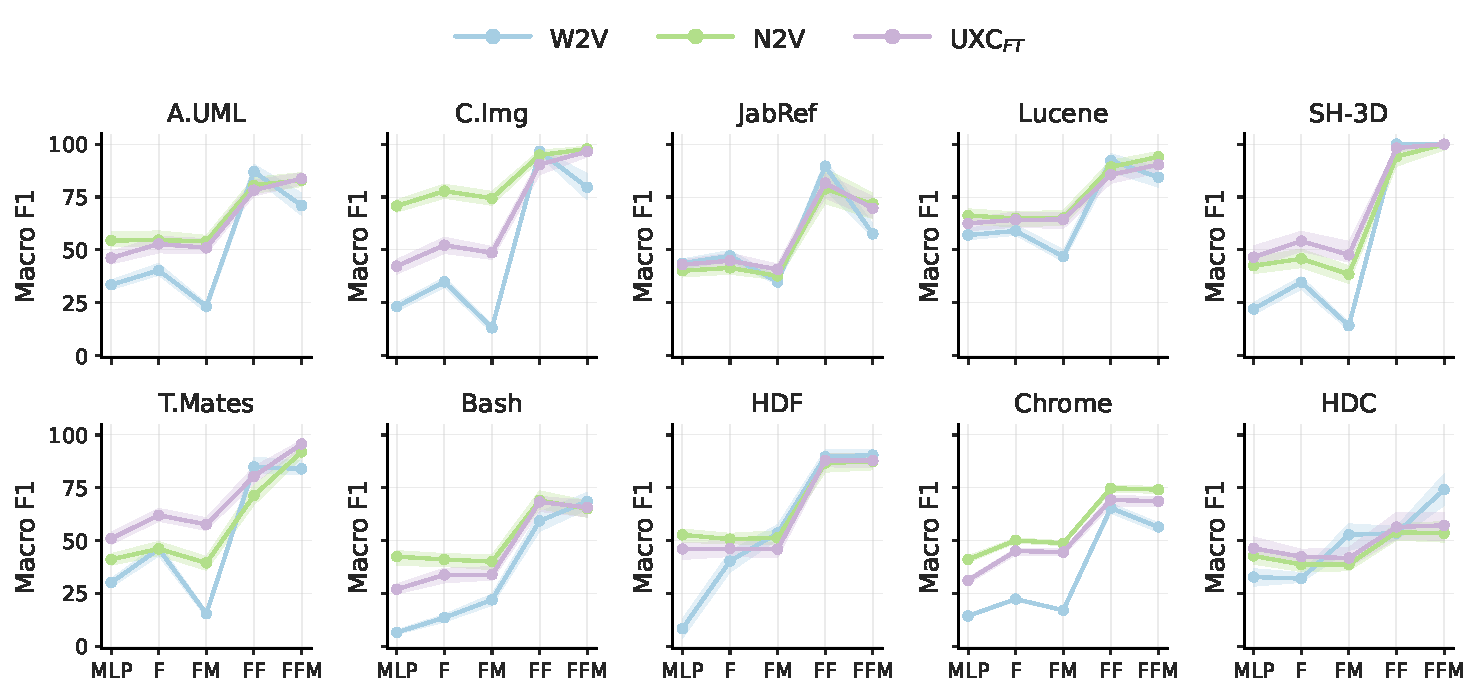
\includegraphics[width=1\textwidth]{Images/RQ2_lineplot_f1_macro.pdf}
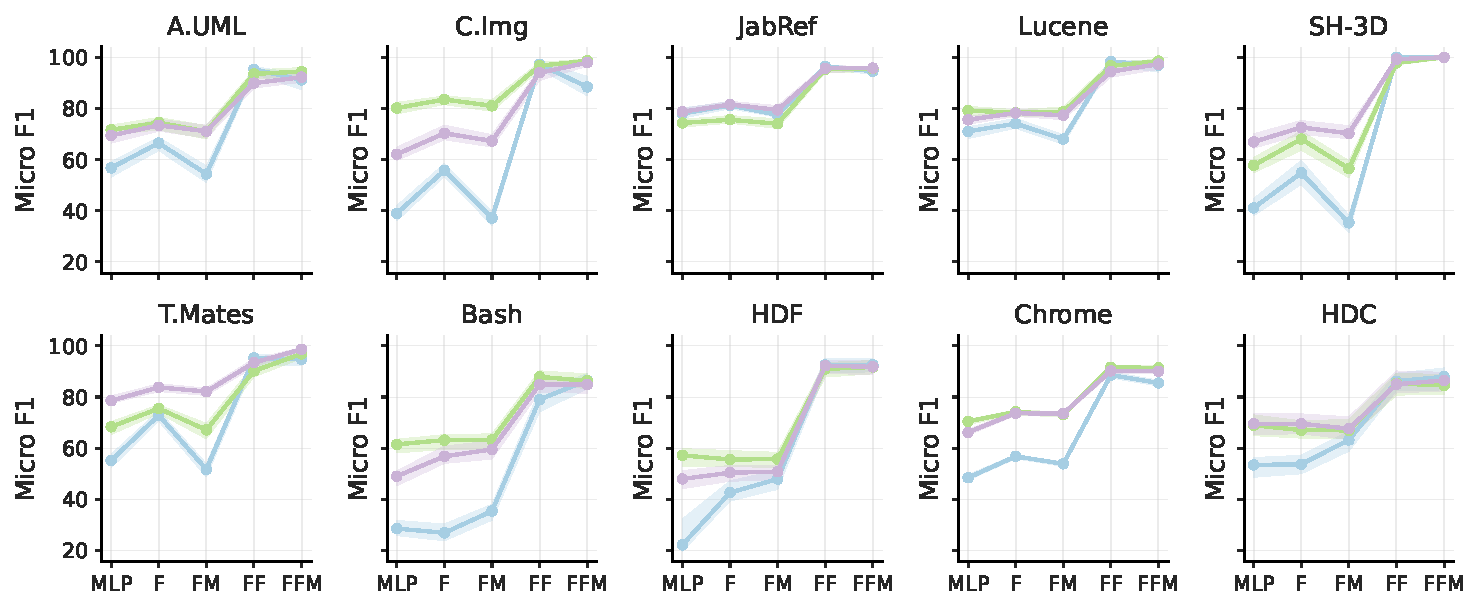
\includegraphics[width=1\textwidth]{Images/RQ2_lineplot_f1_micro.pdf}
\caption{Median macro-F1 (top) and micro-F1 (bottom) for each representation, per system, across the MLP and HGT with increasing graph structure (F, FF, FM, FFM). Shaded areas denote interquartile ranges across the 100 runs. \label{fig:rq2_lineplot}}
\end{figure*}
\begin{table*}[t]
\centering
\caption{Change in macro- and micro-F1 as graph structure is added, by representation. Each row compares the later configuration with the earlier one. Each cell gives the median difference across ten systems in F1 points, followed in parentheses by the number of systems with a positive difference and the numbers of significant positive and negative differences. Shading marks the median difference: blue for gains, purple for losses, and darker for larger changes.\label{tab:rq2_steps}}
\begin{adjustbox}{max width=\textwidth}
\setlength{\tabcolsep}{12pt}
\renewcommand{\arraystretch}{1.2}
\begin{tabular}{lrrrrrr}
\toprule
& \multicolumn{2}{c}{W2V} & \multicolumn{2}{c}{N2V} & \multicolumn{2}{c}{\ft{}} \\
\cmidrule(lr){2-3}\cmidrule(lr){4-5}\cmidrule(lr){6-7}
Step & Macro F1 & Micro F1 & Macro F1 & Micro F1 & Macro F1 & Micro F1 \\
\midrule
F $-$ MLP & \gc{45}+1.6 (6; 6/3) & \gc{45}+1.2 (6; 6/2) & \rc{45}$-$2.9 (1; 1/5) & \rc{70}$-$3.2 (2; 2/6) & \gc{45}+2.9 (8; 4/1) & \gc{25}+0.9 (7; 3/1) \\
FM $-$ F & \gc{45}+1.5 (6; 5/3) & \gc{45}+2.6 (7; 6/3) & \gc{25}+0.9 (6; 4/0) & \gc{45}+2.3 (7; 6/2) & \gc{45}+1.5 (7; 2/2) & \gc{45}+1.8 (8; 6/2) \\
FFM $-$ FF & \gc{100}+11.2 (10; 10/0) & \gc{70}+4.5 (10; 9/0) & \gc{70}+3.3 (8; 5/1) & \gc{45}+2.5 (8; 5/0) & \gc{70}+4.4 (8; 7/0) & \gc{45}+2.5 (10; 6/0) \\
FF $-$ F & \gc{100}+32.9 (10; 10/0) & \gc{100}+33.7 (10; 10/0) & \gc{100}+18.1 (10; 10/0) & \gc{100}+16.7 (10; 10/0) & \gc{100}+27.9 (10; 10/0) & \gc{100}+19.8 (10; 10/0) \\
FFM $-$ FM & \gc{100}+47.2 (10; 10/0) & \gc{100}+37.6 (10; 10/0) & \gc{100}+17.4 (10; 10/0) & \gc{100}+16.9 (10; 10/0) & \gc{100}+36.5 (10; 10/0) & \gc{100}+22.2 (10; 10/0) \\
\bottomrule
\end{tabular}
\end{adjustbox}
\end{table*}

% \begin{table*}[t]
% \centering
% \caption{Changes in Macro and F1 as graph structure is added, by representation. Rows compare the later configuration with the earlier one. $\Delta$ is the median difference across nine systems; $+$ve counts positive differences; $\uparrow/\downarrow$ gives the numbers of significant positive and negative differences, respectively (Wilcoxon signed-rank test, Holm-adjusted, $\alpha=0.05$). Shading marks $\Delta$: blue for gains, purple for losses, darker for larger changes.\label{tab:rq2_steps}}
% \begin{adjustbox}{max width=\textwidth}
% \large
% \begin{tabular}{lrrrrrrrrrrrrrrrrrrr}
% \toprule
% & \multicolumn{6}{c}{W2V} & \multicolumn{6}{c}{N2V} & \multicolumn{6}{c}{\ft{}} \\
% \cmidrule(lr){2-7}\cmidrule(lr){8-13}\cmidrule(lr){14-19}
% & \multicolumn{3}{c}{Macro F1} & \multicolumn{3}{c}{Micro F1}
% & \multicolumn{3}{c}{Macro F1} & \multicolumn{3}{c}{Micro F1}
% & \multicolumn{3}{c}{Macro F1} & \multicolumn{3}{c}{Micro F1} \\
% \cmidrule(lr){2-4}\cmidrule(lr){5-7}
% \cmidrule(lr){8-10}\cmidrule(lr){11-13}
% \cmidrule(lr){14-16}\cmidrule(lr){17-19}
% Step
% & $\Delta$ & $+$ve & $\uparrow/\downarrow$
% & $\Delta$ & $+$ve & $\uparrow/\downarrow$
% & $\Delta$ & $+$ve & $\uparrow/\downarrow$
% & $\Delta$ & $+$ve & $\uparrow/\downarrow$
% & $\Delta$ & $+$ve & $\uparrow/\downarrow$
% & $\Delta$ & $+$ve & $\uparrow/\downarrow$ \\
% \midrule
% F $-$ MLP
% & \gc{45}+1.8 & 6 & 6/2 & \gc{45}+1.5 & 6 & 6/3
% & \rc{45}$-$2.7 & 1 & 1/5 & \rc{45}$-$2.1 & 2 & 2/5
% & \gc{70}+3.7 & 7 & 6/1 & \gc{45}+1.2 & 7 & 7/1 \\
% FM $-$ F
% & \gc{25}+0.5 & 5 & 5/4 & \gc{45}+2.7 & 6 & 6/3
% & \gc{25}+0.1 & 5 & 3/1 & \gc{45}+1.5 & 6 & 6/3
% & \gc{45}+1.5 & 6 & 6/2 & \gc{45}+1.6 & 7 & 7/2 \\
% FFM $-$ FF
% & \gc{100}+10.1 & 9 & 9/0 & \gc{70}+4.0 & 9 & 9/0
% & \gc{45}+1.9 & 7 & 4/1 & \gc{45}+2.0 & 7 & 5/1
% & \gc{70}+3.6 & 7 & 7/0 & \gc{45}+2.4 & 9 & 9/0 \\
% FF $-$ F
% & \gc{100}+29.9 & 9 & 9/0 & \gc{100}+38.7 & 9 & 9/0
% & \gc{100}+19.0 & 9 & 9/0 & \gc{100}+16.4 & 9 & 9/0
% & \gc{100}+27.7 & 9 & 9/0 & \gc{100}+20.6 & 9 & 9/0 \\
% FFM $-$ FM
% & \gc{100}+45.5 & 9 & 9/0 & \gc{100}+38.8 & 9 & 9/0
% & \gc{100}+18.5 & 9 & 9/0 & \gc{100}+18.7 & 9 & 9/0
% & \gc{100}+35.9 & 9 & 9/0 & \gc{100}+20.8 & 9 & 9/0 \\
% \bottomrule
% \end{tabular}
% \end{adjustbox}
% \end{table*}

%_______________

\parg{File-level HGT versus the MLP.} Moving from the MLP to file-level HGT improves Word2Vec and \ft{} more than Node2Vec. For Word2Vec and \ft{}, F improves median macro-F1 by 7.5 and 6.7 points and median micro-F1 by 9.0 and 4.6 points, with positive differences on nine systems for each representation and metric. Word2Vec has no significant losses, while \ft{} has one on HDC macro-F1. For Node2Vec, the corresponding changes are 0.8 and 2.2 points, with positive differences on six and seven systems. Significant losses occur on Lucene and HDC for both metrics and on HDF for macro-F1, but significant gains still outnumber losses (five to three on macro-F1, seven to two on micro-F1).

\parg{Member-level context.} Adding member nodes to F lowers median macro-F1 by 12.2 points for Word2Vec and 1.2 points for both Node2Vec and \ft{}, and median micro-F1 by 4.9, 1.3, and 1.8 points, respectively. Word2Vec shows the largest decline, with large effects on all ten systems. Significant macro-F1 losses outnumber gains for every representation: seven versus three systems for Word2Vec, five versus none for Node2Vec, and six versus one for \ft{}.

Adding member nodes also changes how features enter the model, depending on the representation (Section~\ref{sec:node_features}); for example, the \ft{} member vectors come from an encoder fine-tuned on file-level text. In addition, with one HGT layer, member-level dependencies cannot affect file predictions, so we test two layers at the end of this section. These results therefore concern the evaluated member configuration, not member information in general.

\parg{Folder-level context.}
Adding folder nodes produces the largest and most consistent changes. FF improves over F, and FFM improves over FM, on both metrics for every system and representation. All 120 system--representation--metric comparisons are significant with a large effect. Across the three representations, the median macro-F1 gains range from 25.6 to 44.4 points for FF $-$ F and from 28.9 to 43.0 points for FFM $-$ FM. The corresponding micro-F1 gains range from 16.5 to 32.1 points and from 20.6 to 39.9 points. Each comparison improves in at least 96 of the 100 paired runs.
 
Within the folder-containing configurations, the effect of adding member nodes depends on the representation. FFM improves macro-F1 over FF on six systems each for Node2Vec and \ft{}, with median gains of 1.6 and 1.3 points, but on only three systems for Word2Vec, with a median loss of 4.4 points. For micro-F1, it improves seven, seven, and three systems for Node2Vec, \ft{}, and Word2Vec, with median changes of $+0.8$, $+1.1$, and $-1.0$ points. Significant macro-F1 losses occur on five systems for Word2Vec and on JabRef, Bash, and Chrome for both Node2Vec and \ft{}. For micro-F1, Node2Vec loses significantly only on Bash, and \ft{} on no system.

\parg{Folder nodes and the directory baseline.\label{sec:directory_errors}}
The large gains from adding folder nodes show that directory organization is informative for the evaluated mappings. To examine whether these gains also help files misclassified by directory information alone, we compare FM and FFM with \ft{} features against the directory hierarchy baseline of Section~\ref{sec:dir_predictor}.  FM and FFM differ only in the inclusion of folder nodes, allowing us to compare their performance with and without folder information. Table~\ref{tab:dir_baseline} gives the accuracy of the baseline, FM, and FFM per system, and the accuracy of FM and FFM on the files the baseline gets wrong.

The baseline reaches 89 to 100\% accuracy on every system. Without folder nodes, FM is 14 to 43 points below it. With folder nodes, FFM is within 3 points of the baseline on six systems and within 7 points on A.UML, Bash, and Chrome; it exceeds the baseline only on Lucene. Adding folder nodes therefore brings FFM close to the accuracy of the directory hierarchy baseline on most systems.

Directory membership closely matches module membership: on eight systems, 99 to 100\% of files belong to the majority module of their directory, and only Bash (91.8\%) and HDC (96.1\%) have lower purity. Files that depart from the majority module of their directory are therefore rare on most systems, which limits what the analysis can show about them.

On the files the baseline gets wrong, FFM gets most of them wrong on A.UML, JabRef, Bash, Chrome, and HDC, about 50\% on HDF, and most of them right only on Lucene. Compared with FM, FFM is more accurate on these files on A.UML, HDF, and Lucene, similar on Bash and Chrome, and less accurate on JabRef and HDC. JabRef shows why a higher overall accuracy is not sufficient: FFM improves over FM overall (79.4\% to 95.8\%), but its accuracy on these files falls (45.3\% to 26.3\%). This analysis does not isolate files whose module differs from the majority module of their directory, so it does not show how well FFM handles such exceptions.
\begin{table}[h]
\centering
\caption{\fontsize{9.5}{12}\selectfont Accuracy (\%) of the directory baseline (Dir.) and of HGT with \ft{} features on FM, FFM and FT, median over 100 runs. FT is HGT on the file graph F with binary folder tokens added to the file vector. $n$ is the median number of test files misclassified by the baseline per split; the FM, FFM and FT columns under it report median accuracy on those files over splits with at least one baseline error. Dashes (--) indicate omitted values for systems with no baseline errors in most or all splits. Purity is the share of all files that belong to the majority module of their directory.\label{tab:dir_baseline}}
\begin{adjustbox}{max width=\linewidth}
\begin{tabular}{lrrrrrrrrr}
\toprule
& \multicolumn{4}{c}{Accuracy} & \multicolumn{4}{c}{Files the baseline gets wrong} & \\
\cmidrule(lr){2-5}\cmidrule(lr){6-9}
System & Dir. & FM & FFM & FT & $n$ & FM & FFM & FT & Purity \\
\midrule
A.UML   & 98.5  & 71.0 & 92.2  & 92.5 & 11   & 9.1  & 21.7 & 22.5 & 100.0 \\
C.Img   & 100.0 & 67.3 & 97.9  & 99.3 & 0    & --   & --   & --   & 100.0 \\
JabRef  & 97.2  & 79.4 & 95.8  & 93.4 & 27   & 45.3 & 26.3 & 25.0 & 99.1  \\
Lucene  & 91.5  & 77.4 & 97.3  & 95.1 & 85.5 & 52.9 & 86.9 & 81.7 & 100.0 \\
SH-3D   & 100.0 & 70.3 & 100.0 & 99.3 & 0    & --   & --   & --   & 100.0 \\
T.Mates & 100.0 & 82.1 & 98.6  & 98.8 & 0    & --   & --   & --   & 100.0 \\
Bash    & 91.8  & 59.5 & 84.8  & 85.9 & 21   & 24.6 & 26.1 & 27.8 & 91.8  \\
HDF     & 93.4  & 50.8 & 91.8  & 92.6 & 8    & 27.3 & 50.0 & 40.0 & 100.0 \\
Chrome  & 96.8  & 73.5 & 90.0  & 94.1 & 574  & 19.8 & 20.0 & 23.3 & 99.9  \\
HDC     & 89.1  & 67.6 & 86.5  & 87.4 & 19   & 20.0 & 12.5 & 10.8 & 96.1  \\
\bottomrule
\end{tabular}
\end{adjustbox}
\end{table}

\parg{Effect of two message-passing layers.} All results above use one HGT layer. To test whether this limits the results, we repeated F, FF, FM, and FFM with two layers, using the same labeled sets, representations, and training settings (Table~\ref{tab:rq2_depth}). For Word2Vec, the largest median macro-F1 improvements occur in FM and FFM. For \ft{}, FF improves more than FFM, so the improvement is not specific to member nodes. Node2Vec shows little change in either member-containing configuration, but F is significantly lower on macro-F1 on five systems.

At matched two-layer depth, adding members to F still lowers median macro-F1 for all three representations. Adding members to FF remains negative for Word2Vec, while the small median gain for \ft{} shrinks and that for Node2Vec becomes slightly negative. Folder nodes retain the largest gains: both folder additions improve both metrics on all ten systems for every representation, with significant large effects. Thus, additional depth improves some configurations but does not establish a consistent benefit from adding member nodes.
\begin{table}[h]
\centering
\caption{\fontsize{9}{12}\selectfont Effect of a second message-passing layer on HGT. $\Delta$ is the median over ten systems of the change in median F1 (points) from one to two layers. +ve is the number of systems with a positive change, followed by the numbers with a significant gain ($\uparrow$) and loss ($\downarrow$).  Shading marks comparisons with at least five significant gains and at least twice as many significant gains as losses.\label{tab:rq2_depth}}
\setlength{\tabcolsep}{8pt}
\begin{adjustbox}{max width=\columnwidth}
\begin{tabular}{llrcrc}
\toprule
& & \multicolumn{2}{c}{Macro-F1} & \multicolumn{2}{c}{Micro-F1} \\
\cmidrule(lr){3-4}\cmidrule(lr){5-6}
Input & Graph & $\Delta$ & +ve ($\uparrow$/$\downarrow$) & $\Delta$ & +ve ($\uparrow$/$\downarrow$) \\
\midrule
\multirow{4}{*}{W2V} & F & +0.5 & 6 (3/4) & 0.0 & 6 (4/3) \\
  & FF & \best{+2.4} & \best{8 (6/1)} & \best{+0.5} & \best{6 (6/0)} \\
  & FM & \best{+3.5} & \best{6 (6/3)} & \best{+2.2} & \best{8 (7/2)} \\
  & FFM & \best{+10.3} & \best{6 (6/3)} & \best{+1.1} & \best{6 (6/3)} \\
\midrule
\multirow{4}{*}{N2V} & F & $-$0.6 & 4 (2/5) & $-$0.1 & 4 (2/4) \\
  & FF & \best{+1.8} & \best{7 (5/2)} & +0.4 & 6 (4/3) \\
  & FM & 0.0 & 5 (3/3) & +0.1 & 5 (3/3) \\
  & FFM & +0.3 & 5 (4/3) & $-$0.2 & 3 (2/4) \\
\midrule
\multirow{4}{*}{\ft{}} & F & 0.0 & 6 (2/1) & \best{+0.8} & \best{8 (7/1)} \\
  & FF & \best{+3.4} & \best{8 (8/2)} & \best{+1.4} & \best{10 (7/0)} \\
  & FM & $-$0.2 & 5 (1/2) & 0.0 & 5 (3/3) \\
  & FFM & \best{+2.6} & \best{7 (7/1)} & \best{+1.0} & \best{8 (8/1)} \\
\bottomrule
\end{tabular}
\end{adjustbox}
\end{table}


\begin{GrayBox}{Answer to RQ2.}
The effect on mapping performance depends on what is added and on the representation. Moving from the MLP to file-level HGT improves Word2Vec and \ft{} more than Node2Vec. Member nodes give no consistent gain and often lower performance, most strongly for Word2Vec. Folder nodes provide the largest gains, with significant large effects on all ten systems for all three representations. Both findings remain with two HGT layers. However, the directory hierarchy alone achieves accuracy similar to FFM on most systems. On most systems with directory-baseline errors, FFM misclassifies most of these files, and on some it is less accurate than FM. Strong folder-based scores therefore do not establish reliable performance on directory-baseline errors or on files whose directory location is insufficient or misleading.
\end{GrayBox}
% ========================================
% ----------------- RQ3 ------------------
% ========================================
\subsection{Dependency Neighbors, Predictors, and Aggregation Direction (RQ3)\label{sec:rq3}}

RQ2 shows that the effect of graph context depends on the representation, configuration, and system. However, its comparison of the MLP with file-level HGT changes both the predictor and the availability of dependency messages. RQ3 therefore compares each predictor with dependency neighbors disabled and enabled, using HGT, GAT, and a neighbor MLP (\mlp{}). It also compares directed and undirected aggregation to examine whether the benefit depends on how dependency neighbors are aggregated. We evaluate all three predictors with all four input representations.

Differences are paired changes in F1 points, enabled minus disabled; positive values favor neighbor information. For direction, differences are undirected minus directed; positive values favor undirected neighbors. We report the median paired difference over the 100 splits. With neighbors disabled, the neighbor MLP reduces to the MLP of RQ1, and GAT and HGT receive no dependency messages.

\parg{How does the benefit of dependency neighbors vary across predictors and representations?} Table~\ref{tab:rq3_reps} shows the change in F1 when neighbor information is enabled, for each predictor and input representation. With undirected neighbors, the median change is positive in every cell on both metrics. GAT and the \mlp{} improve on at least eight systems in every cell and are never significantly lower, whereas HGT gains least with every representation and is significantly lower on a few systems with Node2Vec and Word2Vec. With directed neighbors, the median macro-F1 is lower with Node2Vec for all three predictors, by 0.6 to 2.8 points, and significant losses occur on up to six systems. For GAT and the \mlp{}, the gain from undirected neighbors is smallest with Node2Vec and largest with \zs{}.

This comparison differs from RQ2, where file-level message passing (F) is compared with the MLP, which changes the predictor together with the available structure. Here the predictor is fixed, and dependency neighbors are enabled and disabled, so a gain of F over the MLP does not imply that HGT benefits from dependency neighbors. With Node2Vec, for example, F raises the median macro-F1 over the MLP, whereas HGT with directed neighbors is lower than HGT without neighbors.

\begin{table*}[t]
\centering
\caption{Changes in F1 from enabling neighbor information (D$-$off, UD$-$off) and switching from directed to undirected aggregation (UD$-$D), by model and input representation. Each cell reports the median across ten systems of the per-system median paired change over runs, in F1 points. Parentheses follow the format (systems with a positive median change; significant gains/significant losses). D: directed (source-to-target); UD: undirected; off: neighbor information disabled. Blue shading indicates gains and purple indicates losses, with darker shades indicating larger magnitudes.\label{tab:rq3_reps}}

\begin{adjustbox}{max width=\textwidth}
\renewcommand{\arraystretch}{1.1}
\normalsize
\begin{tabular}{llrrrrrrrr}
\toprule
& & \multicolumn{2}{c}{N2V} & \multicolumn{2}{c}{W2V} & \multicolumn{2}{c}{\zs{}} & \multicolumn{2}{c}{\ft{}} \\
\cmidrule(lr){3-4}\cmidrule(lr){5-6}\cmidrule(lr){7-8}\cmidrule(lr){9-10}
Model & Contrast & Macro F1 & Micro F1 & Macro F1 & Micro F1 & Macro F1 & Micro F1 & Macro F1 & Micro F1 \\
\midrule
\multirow{3}{*}{HGT} & D$-$off & \rc{25}$-$0.6 (4; 4/6) & \gc{45}+1.6 (6; 6/4) & \gc{25}+0.2 (5; 4/5) & \gc{45}+1.8 (7; 7/3) & \gc{45}+1.6 (9; 7/0) & \gc{45}+2.7 (10; 10/0) & \gc{25}+0.7 (7; 6/3) & \gc{45}+1.8 (8; 8/0) \\
 & UD$-$off & \gc{25}+0.5 (8; 5/2) & \gc{25}+0.8 (9; 8/0) & \gc{45}+2.9 (7; 7/3) & \gc{70}+4.5 (8; 8/2) & \gc{45}+1.8 (10; 10/0) & \gc{45}+2.5 (10; 10/0) & \gc{25}+0.9 (10; 8/0) & \gc{45}+1.6 (10; 10/0) \\
 & UD$-$D & \gc{25}+0.3 (6; 5/4) & \gc{25}+0.1 (5; 3/4) & \gc{25}+0.7 (7; 4/3) & \gc{45}+1.5 (6; 5/4) & \rc{25}0.0 (5; 4/3) & \gc{25}+0.1 (5; 5/4) & \gc{25}+0.6 (6; 5/3) & \gc{25}+0.2 (5; 4/4) \\
\addlinespace[3pt]

\multirow{3}{*}{GAT} & D$-$off & \rc{45}$-$2.8 (4; 3/6) & \rc{25}$-$0.8 (3; 2/5) & \gc{45}+1.5 (8; 6/2) & \gc{45}+2.4 (7; 7/1) & \gc{70}+3.8 (10; 9/0) & \gc{100}+6.2 (10; 10/0) & \gc{25}+0.7 (6; 4/2) & \gc{45}+2.2 (8; 7/1) \\
 & UD$-$off & \gc{45}+1.4 (9; 8/0) & \gc{45}+1.4 (10; 10/0) & \gc{70}+5.6 (8; 7/0) & \gc{100}+6.7 (8; 8/0) & \gc{100}+8.2 (10; 10/0) & \gc{100}+9.5 (10; 10/0) & \gc{70}+3.8 (10; 8/0) & \gc{70}+4.1 (10; 10/0) \\
 & UD$-$D & \gc{70}+3.8 (7; 6/2) & \gc{45}+2.2 (8; 8/1) & \gc{45}+1.9 (7; 5/3) & \gc{45}+1.6 (7; 5/3) & \gc{70}+3.3 (6; 6/4) & \gc{45}+2.2 (6; 6/2) & \gc{45}+3.0 (6; 6/4) & \gc{45}+1.3 (7; 6/1) \\
\addlinespace[3pt]

\multirow{3}{*}{\mlp{}} & D$-$off & \rc{25}$-$0.6 (4; 4/5) & \gc{25}+0.8 (6; 5/4) & \gc{70}+3.4 (9; 9/1) & \gc{45}+2.7 (9; 8/1) & \gc{70}+4.8 (8; 7/1) & \gc{70}+5.1 (9; 9/0) & \gc{45}+2.8 (7; 6/2) & \gc{45}+2.9 (7; 7/2) \\
 & UD$-$off & \gc{45}+1.2 (10; 8/0) & \gc{45}+1.2 (9; 8/0) & \gc{70}+5.1 (10; 10/0) & \gc{70}+4.9 (10; 10/0) & \gc{100}+7.7 (10; 10/0) & \gc{100}+7.3 (10; 10/0) & \gc{70}+5.8 (10; 10/0) & \gc{70}+4.6 (10; 10/0) \\
 & UD$-$D & \gc{45}+1.6 (6; 6/4) & \gc{25}+0.4 (6; 5/3) & \gc{45}+1.3 (6; 6/3) & \gc{45}+1.9 (6; 6/2) & \gc{70}+3.5 (6; 6/4) & \gc{45}+2.5 (6; 6/4) & \gc{70}+3.1 (6; 6/3) & \gc{45}+1.3 (7; 7/3) \\
\bottomrule
\end{tabular}
\end{adjustbox}
\end{table*}



 % \begin{table*}[thb]
% \centering
% \caption{Change in macro- and micro-F1 when neighbor information is switched on, by input vector. $\Delta$ is the median difference across nine systems; $+$ve counts positive differences; $\uparrow/\downarrow$ gives the numbers of significant positive and negative differences, respectively (Wilcoxon signed-rank test, Holm-adjusted, $\alpha=0.05$). Shading marks $\Delta$: blue for gains, purple for losses, darker for larger changes.\label{tab:rq3_reps}}
% \begin{adjustbox}{max width=\textwidth}
% \large
% \begin{tabular}{llrrrrrrrrrrrrrrrrrrrrrrrr}
% \toprule
% & & \multicolumn{6}{c}{N2V} & \multicolumn{6}{c}{W2V} & \multicolumn{6}{c}{\zs{}} & \multicolumn{6}{c}{\ft{}} \\
% \cmidrule(lr){3-8}\cmidrule(lr){9-14}\cmidrule(lr){15-20}\cmidrule(lr){21-26}
% & & \multicolumn{3}{c}{Macro F1} & \multicolumn{3}{c}{Micro F1}
% & \multicolumn{3}{c}{Macro F1} & \multicolumn{3}{c}{Micro F1}
% & \multicolumn{3}{c}{Macro F1} & \multicolumn{3}{c}{Micro F1}
% & \multicolumn{3}{c}{Macro F1} & \multicolumn{3}{c}{Micro F1} \\
% \cmidrule(lr){3-5}\cmidrule(lr){6-8}
% \cmidrule(lr){9-11}\cmidrule(lr){12-14}
% \cmidrule(lr){15-17}\cmidrule(lr){18-20}
% \cmidrule(lr){21-23}\cmidrule(lr){24-26}
% Model & Sch.
% & $\Delta$ & $+$ve & $\uparrow/\downarrow$
% & $\Delta$ & $+$ve & $\uparrow/\downarrow$
% & $\Delta$ & $+$ve & $\uparrow/\downarrow$
% & $\Delta$ & $+$ve & $\uparrow/\downarrow$
% & $\Delta$ & $+$ve & $\uparrow/\downarrow$
% & $\Delta$ & $+$ve & $\uparrow/\downarrow$
% & $\Delta$ & $+$ve & $\uparrow/\downarrow$
% & $\Delta$ & $+$ve & $\uparrow/\downarrow$ \\
% \midrule

% HGT & sup. & \rc{70}$-$4.6 & 1 & 0/5 & \rc{45}$-$2.0 & 2 & 2/4 & \rc{70}$-$3.9 & 2 & 2/7 & \rc{45}$-$1.0 & 2 & 2/5 & \rc{45}$-$1.2 & 4 & 1/2 & \rc{25}$-$0.2 & 4 & 2/1 & \rc{70}$-$3.9 & 4 & 0/3 & \rc{45}$-$1.7 & 3 & 1/3 \\
%  & self. & \rc{70}$-$4.8 & 0 & 0/5 & \rc{45}$-$2.4 & 3 & 1/4 & \rc{70}$-$3.6 & 2 & 2/7 & \rc{45}$-$2.0 & 3 & 2/5 & \rc{45}$-$1.3 & 2 & 0/0 & \gc{25}+0.2 & 5 & 1/1 & \rc{45}$-$2.2 & 2 & 0/3 & \rc{45}$-$1.2 & 3 & 1/2 \\
% \addlinespace[3pt]
% \multirow{2}{*}{\shortstack[l]{HGT\\-UT}} & sup. & \gc{25}+0.6 & 5 & 2/1 & \gc{25}+0.9 & 7 & 2/0 & \gc{45}+2.6 & 6 & 4/1 & \gc{70}+4.0 & 7 & 7/1 & \gc{45}+1.6 & 9 & 8/0 & \gc{70}+3.1 & 9 & 9/0 & \gc{25}+0.9 & 9 & 2/0 & \gc{45}+1.4 & 9 & 6/0 \\
%  & self. & \gc{25}+0.4 & 6 & 0/1 & \gc{45}+1.2 & 8 & 3/0 & \gc{45}+1.7 & 6 & 2/0 & \gc{70}+3.9 & 7 & 7/0 & \gc{45}+2.1 & 8 & 6/0 & \gc{70}+3.1 & 9 & 8/0 & \gc{45}+1.8 & 9 & 2/0 & \gc{45}+2.0 & 9 & 5/0 \\
% \addlinespace[3pt]
% GAT & sup. & \gc{45}+1.1 & 8 & 3/0 & \gc{45}+1.6 & 9 & 9/0 & \gc{70}+5.7 & 8 & 3/0 & \gc{100}+6.4 & 9 & 6/0 & \gc{100}+7.7 & 9 & 7/0 & \gc{100}+10.5 & 9 & 9/0 & \gc{70}+4.2 & 7 & 4/0 & \gc{70}+4.4 & 9 & 7/0 \\
%  & self. & \gc{70}+3.2 & 9 & 3/0 & \gc{45}+2.9 & 8 & 7/0 & \gc{70}+3.7 & 7 & 3/0 & \gc{100}+6.9 & 7 & 6/0 & \gc{100}+8.0 & 8 & 8/0 & \gc{100}+8.9 & 9 & 9/0 & \gc{70}+4.2 & 8 & 4/0 & \gc{70}+4.2 & 8 & 4/0 \\
% \addlinespace[3pt]
% MLP & sup. & \gc{25}+0.7 & 8 & 4/0 & \gc{45}+1.4 & 8 & 5/0 & \gc{70}+4.4 & 8 & 6/0 & \gc{70}+4.4 & 8 & 5/0 & \gc{100}+6.9 & 9 & 8/0 & \gc{70}+5.2 & 9 & 9/0 & \gc{70}+4.0 & 8 & 4/0 & \gc{70}+4.5 & 9 & 5/0 \\
%  & self. & \gc{45}+2.6 & 8 & 5/0 & \gc{45}+2.8 & 8 & 6/0 & \gc{70}+3.6 & 9 & 6/0 & \gc{70}+4.6 & 9 & 5/0 & \gc{100}+6.8 & 8 & 6/0 & \gc{100}+6.9 & 9 & 9/0 & \gc{100}+6.3 & 9 & 5/0 & \gc{70}+4.6 & 9 & 8/0 \\
% \bottomrule
% \end{tabular}
% \end{adjustbox}
% \end{table*}


% % --- Table B
% \begin{table*}[thb]
% \centering
% \caption{Change in macro- and micro-F1 when neighbor information is switched on, by input vector. $\Delta$ is the median difference across nine systems; $+$ve counts positive differences; $\uparrow/\downarrow$ gives the numbers of significant positive and negative differences, respectively (Wilcoxon signed-rank test, Holm-adjusted, $\alpha=0.05$). Shading marks $\Delta$: blue for gains, purple for losses, darker for larger changes.\label{tab:rq3_reps}}
% \begin{adjustbox}{max width=\textwidth}
% \large
% \begin{tabular}{llrrrrrrrrrrrrrrrrrr}
% \toprule
% & & \multicolumn{6}{c}{N2V} & \multicolumn{6}{c}{W2V} & \multicolumn{6}{c}{\ft{}} \\
% \cmidrule(lr){3-8}\cmidrule(lr){9-14}\cmidrule(lr){15-20}
% & & \multicolumn{3}{c}{Macro F1} & \multicolumn{3}{c}{Micro F1}
% & \multicolumn{3}{c}{Macro F1} & \multicolumn{3}{c}{Micro F1}
% & \multicolumn{3}{c}{Macro F1} & \multicolumn{3}{c}{Micro F1} \\
% \cmidrule(lr){3-5}\cmidrule(lr){6-8}
% \cmidrule(lr){9-11}\cmidrule(lr){12-14}
% \cmidrule(lr){15-17}\cmidrule(lr){18-20}
% Model & Sch.
% & $\Delta$ & $+$ve & $\uparrow/\downarrow$
% & $\Delta$ & $+$ve & $\uparrow/\downarrow$
% & $\Delta$ & $+$ve & $\uparrow/\downarrow$
% & $\Delta$ & $+$ve & $\uparrow/\downarrow$
% & $\Delta$ & $+$ve & $\uparrow/\downarrow$
% & $\Delta$ & $+$ve & $\uparrow/\downarrow$ \\
% \midrule

% HGT & sup. & \rc{70}$-$4.6 & 1 & 0/5 & \rc{45}$-$2.0 & 2 & 2/4 & \rc{70}$-$3.9 & 2 & 2/7 & \rc{45}$-$1.0 & 2 & 2/5 & \rc{70}$-$3.9 & 4 & 0/3 & \rc{45}$-$1.7 & 3 & 1/3 \\
%  & self. & \rc{70}$-$4.8 & 0 & 0/5 & \rc{45}$-$2.4 & 3 & 1/4 & \rc{70}$-$3.6 & 2 & 2/7 & \rc{45}$-$2.0 & 3 & 2/5 & \rc{45}$-$2.2 & 2 & 0/3 & \rc{45}$-$1.2 & 3 & 1/2 \\
% \addlinespace[3pt]
% \uhgt{} & sup. & \gc{25}+0.6 & 5 & 2/1 & \gc{25}+0.9 & 7 & 2/0 & \gc{45}+2.6 & 6 & 4/1 & \gc{70}+4.0 & 7 & 7/1 & \gc{25}+0.9 & 9 & 2/0 & \gc{45}+1.4 & 9 & 6/0 \\
%  & self. & \gc{25}+0.4 & 6 & 0/1 & \gc{45}+1.2 & 8 & 3/0 & \gc{45}+1.7 & 6 & 2/0 & \gc{70}+3.9 & 7 & 7/0 & \gc{45}+1.8 & 9 & 2/0 & \gc{45}+2.0 & 9 & 5/0 \\
% \addlinespace[3pt]
% GAT & sup. & \gc{45}+1.1 & 8 & 3/0 & \gc{45}+1.6 & 9 & 9/0 & \gc{70}+5.7 & 8 & 3/0 & \gc{100}+6.4 & 9 & 6/0 & \gc{70}+4.2 & 7 & 4/0 & \gc{70}+4.4 & 9 & 7/0 \\
%  & self. & \gc{70}+3.2 & 9 & 3/0 & \gc{45}+2.9 & 8 & 7/0 & \gc{70}+3.7 & 7 & 3/0 & \gc{100}+6.9 & 7 & 6/0 & \gc{70}+4.2 & 8 & 4/0 & \gc{70}+4.2 & 8 & 4/0 \\
% \addlinespace[3pt]
% MLP & sup. & \gc{25}+0.7 & 8 & 4/0 & \gc{45}+1.4 & 8 & 5/0 & \gc{70}+4.4 & 8 & 6/0 & \gc{70}+4.4 & 8 & 5/0 & \gc{70}+4.0 & 8 & 4/0 & \gc{70}+4.5 & 9 & 5/0 \\
%  & self. & \gc{45}+2.6 & 8 & 5/0 & \gc{45}+2.8 & 8 & 6/0 & \gc{70}+3.6 & 9 & 6/0 & \gc{70}+4.6 & 9 & 5/0 & \gc{100}+6.3 & 9 & 5/0 & \gc{70}+4.6 & 9 & 8/0 \\
% \bottomrule
% \end{tabular}
% \end{adjustbox}
% \end{table*}


\parg{Does the direction of neighbor aggregation matter?} Undirected aggregation gives the higher median in almost every cell of Table~\ref{tab:rq3_reps}, which raises the question of whether it is better on every system. Figure~\ref{fig:rq3_direction} compares the two directions per system. It is not: the change from directed to undirected aggregation is positive on only five to eight systems per cell, and significant changes occur in both directions. On macro-F1, SH-3D, T.Mates, and JabRef score higher with directed aggregation in all 12 cells, and C.Img in eight. Lucene, Bash, Chrome, and HDC score higher with undirected aggregation in all 12 cells, and A.UML and HDF in 11. The differences reach 14.6 points for undirected aggregation (Bash, Word2Vec, \mlp{}) and 8.7 points for directed aggregation (T.Mates, Word2Vec, \mlp{}). Micro-F1 gives the same pattern for seven systems, whereas JabRef, C.Img, and A.UML are mixed. Undirected neighbors also add the reverse edges, so these results do not separate the direction of propagation from the larger neighborhood.

\begin{figure}[t]
\centering
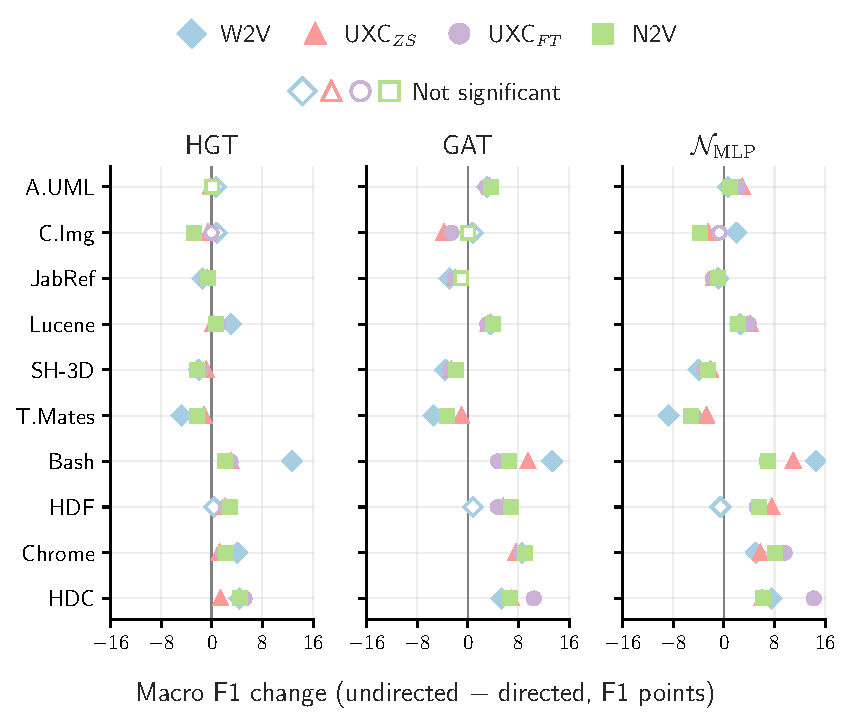
\includegraphics[width=1\columnwidth]{Images/rq3_direction_f1_macro.pdf}
\caption{Change in macro-F1, in F1 points, from directed to undirected aggregation (undirected $-$ directed) for each predictor and input representation; negative values mean directed aggregation scored higher. Each point is the median over 100 paired splits; hollow markers are not significant.\label{fig:rq3_direction}}
\end{figure}

\parg{Which predictor scores highest?} Figure~\ref{fig:rq3_agg} pools the ten systems with undirected neighbors: each point is the median of one system and the boxes show the spread across systems. GAT has the highest median macro-F1 with every representation and the highest median micro-F1 with every representation except Node2Vec, where HGT is marginally higher. GAT also scores highest most often: in each split we count which of the four predictors scores highest, and GAT has the largest share of wins, averaged over systems, with every representation and on both metrics. All three predictors with neighborhood aggregation exceed the MLP without neighbors in every median comparison. As without neighbors, \ft{} has the highest median macro-F1 across systems for every predictor, with GAT and \ft{} giving the highest scores overall.

Most of the variation in F1 lies between systems and not between runs of one system. The choice of predictor matters most for Word2Vec and \zs{}, the two representations without dependency information, and less for Node2Vec and \ft{}.

\begin{figure*}[h]
\centering
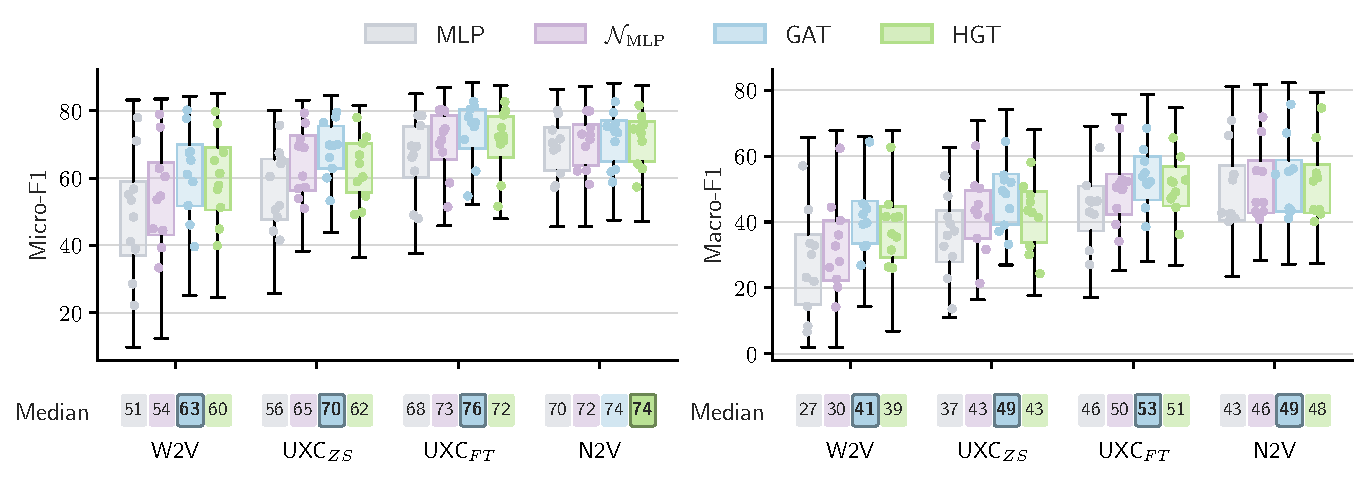
\includegraphics[width=0.98\textwidth]{Images/rq3_fig_compare_undirected.pdf}
\caption{Micro-F1 (left) and macro-F1 (right) of the MLP, \mlp{}, GAT, and HGT with undirected neighbors, by input representation. Each point is the median of one system over 100 runs; boxes show the spread across systems, and the values below are the median of medians across systems, with the highest in each group in bold.\label{fig:rq3_agg}}
\end{figure*}

\begin{GrayBox}{Answer to RQ3.}
Dependency neighbors do not benefit all predictors equally. With undirected aggregation, median changes are positive for every predictor and representation, but GAT and the \mlp{} improve more consistently across systems than HGT, which shows significant losses in some cases. Directed aggregation is less reliable, particularly with Node2Vec, where median macro-F1 decreases for all three predictors. Although undirected aggregation generally gives larger gains, it is not preferable on every system: several systems consistently favor directed aggregation across predictors and representations. These comparisons also change neighborhood size, so they do not isolate direction alone. With undirected neighbors, GAT has the highest median macro-F1 across systems for every representation, and \ft{} remains the strongest representation by this measure for every predictor.
\end{GrayBox}
\section{Discussion\label{sec:discussion}}
The research questions examine where architectural signal resides and how a mapping model can use it. RQ1 compares file representations before message passing, RQ2 examines file, member, and folder context and compares the folder gains with a directory-based rule, and RQ3 examines how predictor choice and aggregation direction affect the contribution of dependency neighbors. This section discusses these findings together.

\subsubsection*{Dependency Information in File Representations}
Dependency information can support mapping before message passing, through the graph position encoded by Node2Vec or through dependency-guided adaptation of a code encoder. The advantage of these representations over Word2Vec, and of fine-tuned UniXcoder over its zero-shot counterpart, suggests that dependency information is useful beyond what the evaluated lexical and pretrained code representations provide. The representations also differ in training, vector size, and source content, so these comparisons are between representation pipelines and not between isolated information sources.

The usefulness of this signal varies with the relation between dependency structure and the reference architecture. Node2Vec’s micro-F1 is lower on the three least homophilic systems, SH-3D, HDF, and T.Mates (Table~\ref{tab:datasets}), with a median of $58$ compared with $72$ on the remaining seven. Node2Vec learns dependency proximity from files that co-occur on random walks, without using the GT mapping. When dependencies frequently cross module boundaries, files from different modules may co-occur on walks and receive similar vectors, making the modules harder to distinguish.

The advantage of fine-tuned UniXcoder over Node2Vec on SH-3D and T.Mates suggests that code content may provide complementary evidence in these mixed neighborhoods. HDF does not follow this pattern, so low homophily alone does not explain their relative performance; HDF is also the smallest system, and every representation has comparatively low micro-F1 on it. Homophily is used here to interpret the observed pattern, not to select a representation, since computing it requires the reference mapping.

Encoding dependencies in the initial representation and aggregating dependency neighbors during mapping are two uses of the same information source, and the second does not necessarily replace the first. With undirected aggregation, the median gains are generally larger for Word2Vec and zero-shot UniXcoder than for Node2Vec and fine-tuned UniXcoder, yet fine-tuned UniXcoder still has the highest median macro-F1 for every predictor. Conversely, useful dependency information in a representation does not guarantee a benefit from further aggregation: RQ3 shows that this benefit depends on both aggregation direction and predictor choice.

\subsubsection*{Folder Organization and Architectural Exceptions}
The gains from adding folder nodes in RQ2 show that directory organization helps reproduce the reference mapping. They do not show that this information must reach a file through message passing over folder nodes, since supplying the same information directly in the file vector matches or exceeds the accuracy of folder nodes on most systems. Extending a directory assignment is also different from identifying files that depart from it. Comparing FM, FFM, and FD on the directory baseline's errors helps assess this distinction (Section~\ref{sec:directory_errors}), but does not isolate architectural exceptions from errors caused by missing local supervision.

Lucene and HDF have pure directories under the reference mapping, so their baseline errors do not reflect conflicts between directory and module membership. They may instead arise from directories without labeled examples, although the table does not establish this. FFM recovers most baseline errors on Lucene and half on HDF, but only about a fifth on A.UML, whose directories are also pure. Directory purity therefore does not ensure that folder nodes recover baseline errors.

Bash and HDC have mixed directories. On baseline errors, FFM is similar to FM on Bash and less accurate on HDC. JabRef further illustrates why overall gains are insufficient: adding folder context raises overall accuracy while lowering accuracy on baseline errors.

The directory rule serves as a reference point for interpreting the learned models. Where directory organization closely follows the architecture, it already reproduces most of the mapping. On most evaluated systems, the added modeling complexity therefore brings little accuracy over the rule. Evaluating the additional value of a learned mapper requires examining both files in directories without labeled examples and files whose module differs from their directory's majority module.

\subsubsection*{Dependency Neighbors and Aggregation Direction}

The benefit of dependency neighbors depends on how the predictor aggregates them. With undirected aggregation, HGT gains least, while GAT achieves the highest median macro-F1 with every representation, although differences between predictors are small relative to variation across systems. GAT and HGT differ in their attention formulations and parameterizations, so the comparison does not isolate why GAT performs better. These findings concern the evaluated file-level predictors, not the usefulness of dependency types in general. RQ2 uses HGT for the folder- and member-aware configurations; whether the folder gains persist with other predictors remains untested.

The preferred aggregation direction appears to depend more on the system than on the predictor or representation, although the pattern is not uniform across metrics. Undirected aggregation generally gives larger gains, but several systems consistently favor directed aggregation. Agreement across predictors and representations describes the stability of these system-level preferences rather than providing independent evidence, since the comparisons share systems and splits.

Undirected aggregation adds reverse edges, so the comparison does not isolate propagation direction from neighborhood size. A reversed-edges-only setting would help distinguish these effects and remains for future work.

With Node2Vec, directed aggregation lowers median macro-F1 for all three predictors. Since its vectors were learned on an undirected graph, this may reflect a mismatch between the neighborhoods encoded during initialization and those used during prediction, but this explanation remains untested.

\subsubsection*{Connectivity and Neighbor Information}
Connectivity describes how much neighboring context is available, measured here by average node degree, while homophily describes whether linked files share a module. Few neighbors limit the context available to shallow message passing, whereas Node2Vec can encode more distant context through random walks. Limited connectivity may therefore constrain the benefit of additional aggregation even when the initial structural representation remains useful.

With Node2Vec and undirected aggregation, no predictor changes significantly on Bash and HDC, the two lowest-degree systems. The depth analysis is also consistent with this interpretation: higher average degree is associated with larger gains from a second message-passing layer, particularly in FFM.

Connectivity may also help explain the effect of aggregation direction. T.Mates and SH-3D combine low homophily with high average degree and favor directed aggregation in RQ3. Bash and HDC favor undirected aggregation, as does HDF, which has low homophily but much lower average degree than T.Mates and SH-3D. Reverse edges may supply missing context in sparse neighborhoods but introduce additional cross-module context in dense, low-homophily neighborhoods. This mechanism remains untested: the ten-system comparison cannot separate connectivity from homophily, system size, or label scarcity.

\subsubsection*{Implications for Evaluation}
Evaluation should establish what the input representation already provides, then isolate access to neighborhood information within a fixed predictor. Comparing a GNN model with an MLP changes both the predictor and the use of dependency-neighborhood aggregation. Enabling and disabling neighborhood aggregation within the same predictor family, while keeping the file representations fixed, provides a more targeted comparison. For the neighbor MLP, this comparison includes an increase in input width and parameter count. The same applies to folder information: a comparison of graph variants should include a model that receives that information directly as file features.

Micro-F1 and macro-F1 should be read together, since correctly mapping more files does not necessarily improve performance across modules. For tools intended to identify architectural exceptions, aggregate scores should also be accompanied by performance on files whose module differs from the majority module of their directory.

The intended use also matters. If mapping supports code reorganization, the existing directory structure may be something to reconsider rather than reproduce. Strong performance based on that structure does not establish which information would remain useful when the organization changes. The present study does not test this setting, but motivates evaluating information sources against the intended task rather than treating any representation or predictor as generally preferable.

\section{Related Work\label{sec:work}}

Architecture recovery and code-to-architecture mapping both infer a system's modular structure from implementation artifacts, such as static dependencies, code semantics, and directory organization. Recovery produces a decomposition without a reference architecture, while mapping assigns entities to the modules of a given one. We evaluate mapping and draw on recovery research for representations of dependencies, lexical content, and project organization.

Recovery techniques have historically been built around one dominant signal: dependency graphs, partitioned by search-based optimization~\cite{bunch,bunch_sahc_nahc,dagc,wca,mca_eca} or clustering~\cite{cct,hcc_2019,limbo,fca,neighborhood_tree_2019,gma_2021}, identifiers and comments~\cite{arc,zbr,risi2012fold,kargar2017semantic}, or file names and paths~\cite{file_clustering}. Each signal is noisy in isolation, since shared utilities introduce cross-module edges and reused terminology mixes entities from many modules, so hybrid methods combine sources~\cite{sc_misra,escrc,nsga3,sadat2019multi,ensemble_recovery,evol,sade,sarif}.

Mapping began with orphan adoption~\cite{tzerpos1997orphan} and the attraction functions of HuGMe~\cite{christl2005equipping,christl2007automated}, and later varied the signal and the learner: textual similarity~\cite{bittencourt_IR}, supervised classifiers~\cite{bibi2016supervised}, and semi-supervised Naive Bayes combining lexical and dependency-derived information~\cite{olsson2019semi,olsson2022automatically}. Text-based approaches compare classifiers for module assignment~\cite{florean2021textclassifierscomparison}, recommend mappings from natural-language architecture descriptions~\cite{InMap}, or integrate package- and class-level granularity~\cite{sinkala2023integrated}. More recent work uses TF-IDF, GloVe, and LLM representations~\cite{johansson2024mapping}, extracts architectural concepts from documentation and code~\cite{fuchss2025enabling}, or prompts LLMs to map implementation units to a reference architecture, which faces context-size limits and repeated processing costs on large codebases~\cite{rukmono_deductive}. Johansson and Caporuscio map functions and files to textual module descriptions with pre-trained embeddings and find files classified more reliably than functions, with performance associated with vocabulary overlap and class separability~\cite{johansson2025mapping}.

Representation-learning work on recovery encoded one or two sources at a time. NEGAR clusters Node2Vec embeddings of the dependency graph alone~\cite{negar}. Jabeen et al.~\cite{structsar} study dependencies alone and with folder organization, comparing random walk-based methods and variational graph autoencoders. GAER~\cite{gaer}, a graph autoencoder, and ARL~\cite{arl_2026}, a contrastively trained GAT, each fix folder and identifier tokens into one encoding without comparing alternatives. For mapping, GNNs were evaluated on homogeneous and dependency-type-aware graphs without folder or member nodes and without separating graph contribution from feature contribution~\cite{jabeen2025graph}. Its extension combines Word2Vec identifier embeddings and binary bag-of-words representations of folder path tokens with dependencies in one model~\cite{c2a_mapping}.

These approaches motivate our distinction between representing an information source and using it during prediction. Text-based mapping reports weaker results for functions than for files~\cite{johansson2026mapping}, but does not examine whether member information helps as context for the file. Our comparisons span lexical, structural, and contextual inputs but retain differences in their training procedures and feature content, so the matched dependency controls and directory-error analyses assess specific design choices and do not turn the broader comparison into an isolated ranking of information sources.
\section{Threats to Validity\label{sec:threats}}

\parg{Generalizability:} We evaluate ten open-source systems in Java, C, and C++, each with one reference architecture. The findings may not extend to other systems or alternative architectural decompositions. The study is transductive: representation learning and graph processing can use unlabeled test nodes and their edges. It therefore does not establish performance on newly arriving files outside the observed graph or on maintaining a mapping as the system evolves. Other information sources, including change history and dynamic dependencies, are outside the evaluated scope.

\parg{Dependencies and reference mappings:} Dependencies are extracted using static analysis, which may miss or misresolve dependencies. Preprocessing and build configuration can also affect the dependencies available for analysis. Because predictors that use neighbors depend on the extracted graph, such errors can affect their predictions. Models with neighbors enabled and disabled are trained separately. Their comparison therefore measures the effect of training with access to neighbor information, rather than removing neighbors from a fixed trained model.

We made a best-effort attempt to identify and obtain the source versions corresponding to the published mappings, using the available version information and documentation. Despite these efforts, some mismatches between the analyzed file sets and the mappings remain. These may reflect incomplete documentation of the original source versions or build configurations, which limits our ability to establish an exact correspondence between the analyzed source code and the published mappings.

Files can plausibly belong to more than one module, and annotators may assign them differently. Because the initial labeled set is sampled from the same mapping used for evaluation, an incorrect assignment can both mislead the model during training and penalize an architecturally plausible prediction.

\parg{Experimental variation:} We use 100 runs per configuration. These runs reuse the same systems and can include the same files, so they are not independent samples. With this many runs, small differences can reach statistical significance, so we report results per system and include effect sizes to distinguish the magnitude of a difference from its significance. The comparisons were not fixed in advance, so the analyses are exploratory and may favor patterns specific to this benchmark.

The runs use different initial labeled sets, but the contribution of stochastic model training to the observed variation was not assessed separately. Input representations were generated once per system and reused across runs, so variation arising from their generation was not assessed. The seeds governing model initialization and training were not retained, limiting exact reproducibility. Cliff's $\delta$ treats the paired scores as two independent groups, so it describes the separation of the two score distributions and not the paired differences.

\parg{Interpretation of results:} Performance measures agreement with the reference architecture, not whether a prediction is the only architecturally reasonable assignment. Folder organization may reflect the same decisions used to define that architecture, so strong directory-based predictions do not by themselves demonstrate recovery of architectural intent. The directory-error analysis applies only where the directory baseline makes errors, which excludes C.Img, SH-3D, and T.Mates in most or all splits, and it does not isolate files whose module differs from the majority module of their directory.
Message-passing depth was varied only for HGT in RQ2, with one and two layers, so the results do not show how deeper models or other predictors respond. It reports accuracy only, so it does not show how performance differs between small and large modules.

Relationships between performance and structural properties are reported as associations, not causal effects, since the benchmark does not allow these properties to be separated from one another or from system size and label availability. The fine-tuning gain is that of the whole dependency-guided procedure, since no alternative adaptation objective was evaluated, so it is not attributed to dependency topology alone.

\section{Conclusion\label{sec:conclusion}}

This study examines how code text, static dependencies, folder organization, and member-level information contribute to code-to-architecture mapping on ten systems. The findings show that mapping performance depends not only on which information is available but also on how it is represented and used.

Representations that encode dependency information generally outperform the evaluated lexical and zero-shot code representations. Node2Vec and dependency-guided fine-tuned UniXcoder outperform Word2Vec on most systems, and fine-tuning improves UniXcoder over its zero-shot counterpart on nearly all systems. However, neither Node2Vec nor fine-tuned UniXcoder is consistently best across systems.

Folder nodes produce the largest and most consistent gains within the HGT variants, but a directory rule using the same labeled files reaches similar accuracy on most systems, and folder paths supplied as file features match or exceed folder nodes on most systems. These gains do not consistently translate into better predictions on files the rule assigns incorrectly. Member nodes provide no consistent improvement with one or two HGT layers, and their effects cannot generally be separated from changes in feature construction and placement. These structural findings are specific to HGT; whether they persist with other predictors remains untested.

Keeping the input representations fixed while enabling and disabling access to dependency-neighborhood information shows that neighbor aggregation can complement representations that already encode dependencies. With undirected aggregation, the median change across systems is positive on both metrics for every predictor and representation. In this setting, GAT achieves the highest median macro-F1, while HGT gains the least. The better aggregation direction varies between systems, although the experiments do not isolate propagation direction from neighborhood size. Evaluation should therefore distinguish information already encoded in the representations from the contribution of neighborhood access. The findings support assessing these contributions for the intended mapping task, rather than treating any representation or predictor as generally preferable.

\parg{Future work.} Future research could clarify how different aspects of graph context contribute to the observed differences. Comparing incoming, outgoing, and combined neighborhoods at matched sizes would help distinguish the effects of propagation direction and neighborhood size. Adding member nodes while preserving each file's own features would help separate the effects of graph structure and feature placement. Another direction is configuration selection on unfamiliar systems. Homophily, which helped interpret the system differences, requires reference module assignments, so selection rules based on properties observable in the dependency graph alone could be developed on some systems and evaluated on others. Finally, a model trained on one version could be evaluated on new and changed files in later versions without retraining, to test whether the learned information supports mapping as systems evolve.


\bibliographystyle{ACM-Reference-Format}
\bibliography{References}

\end{document}